%===============================================================================
% LaTeX sjabloon voor de bachelorproef toegepaste informatica aan HOGENT
% Meer info op https://github.com/HoGentTIN/latex-hogent-report
%===============================================================================

\documentclass[dutch,dit,thesis]{hogentreport}

% TODO:
% - If necessary, replace the option `dit`' with your own department!
%   Valid entries are dbo, dbt, dgz, dit, dlo, dog, dsa, soa
% - If you write your thesis in English (remark: only possible after getting
%   explicit approval!), remove the option "dutch," or replace with "english".

\usepackage{lipsum} % For blind text, can be removed after adding actual content

%% Pictures to include in the text can be put in the graphics/ folder
\graphicspath{{../graphics/}}

%% For source code highlighting, requires pygments to be installed
%% Compile with the -shell-escape flag!
%% \usepackage[chapter]{minted}
%% If you compile with the make_thesis.{bat,sh} script, use the following
%% import instead:
\usepackage[chapter,outputdir=../output]{minted}
\usemintedstyle{solarized-light}


%% Formatting for minted environments.
\setminted{%
    autogobble,
    frame=lines,
    breaklines,
    linenos,
    tabsize=4
}

\usepackage{listings}
\usepackage{xcolor}

\lstdefinelanguage{PowerShell}{
    morekeywords={
        function,param,if,else,foreach,return,try,catch,
        Import-Module,Write-Host,Write-Output
    },
    sensitive=false,
    morecomment=[l]{\#},
    morestring=[b]"
}

%% Ensure the list of listings is in the table of contents
\renewcommand\listoflistingscaption{%
    \IfLanguageName{dutch}{Lijst van codefragmenten}{List of listings}
}
\renewcommand\listingscaption{%
    \IfLanguageName{dutch}{Codefragment}{Listing}
}
\renewcommand*\listoflistings{%
    \cleardoublepage\phantomsection\addcontentsline{toc}{chapter}{\listoflistingscaption}%
    \listof{listing}{\listoflistingscaption}%
}

% Other packages not already included can be imported here



%%---------- Document metadata -------------------------------------------------
% TODO: Replace this with your own information
\author{Ewout Van Mullem}
\supervisor{Dhr. Thomas Aelbrecht}
\cosupervisor{Dhr. Hans Van Mingeroet}
\title[]%
    {Automatisatie van het onboarding en -offboardingsproces binnen het gemeentebestuur van Berlare}
\academicyear{\advance\year by -1 \the\year--\advance\year by 1 \the\year}
\examperiod{1}
\degreesought{\IfLanguageName{dutch}{Professionele bachelor in de toegepaste informatica}{Bachelor of applied computer science}}
\partialthesis{false} %% To display 'in partial fulfilment'
%\institution{Internshipcompany BVBA.}

%% Add global exceptions to the hyphenation here
\hyphenation{back-slash}

%% The bibliography (style and settings are  found in hogentthesis.cls)
\addbibresource{bachproef.bib}            %% Bibliography file
\addbibresource{../voorstel/voorstel.bib} %% Bibliography research proposal
\defbibheading{bibempty}{}

%% Prevent empty pages for right-handed chapter starts in twoside mode
\renewcommand{\cleardoublepage}{\clearpage}

\renewcommand{\arraystretch}{1.2}

%% Content starts here.
\begin{document}

%---------- Front matter -------------------------------------------------------

\frontmatter

\hypersetup{pageanchor=false} %% Disable page numbering references
%% Render a Dutch outer title page if the main language is English
\IfLanguageName{english}{%
    %% If necessary, information can be changed here
    \degreesought{Professionele Bachelor toegepaste informatica}%
    \begin{otherlanguage}{dutch}%
       \maketitle%
    \end{otherlanguage}%
}{}

%% Generates title page content
\maketitle
\hypersetup{pageanchor=true}

%%=============================================================================
%% Voorwoord
%%=============================================================================

\chapter*{\IfLanguageName{dutch}{Woord vooraf}{Preface}}%
\label{ch:voorwoord}

%% TODO:
%% Het voorwoord is het enige deel van de bachelorproef waar je vanuit je
%% eigen standpunt (``ik-vorm'') mag schrijven. Je kan hier bv. motiveren
%% waarom jij het onderwerp wil bespreken.
%% Vergeet ook niet te bedanken wie je geholpen/gesteund/... heeft

Het schrijven van deze bachelorproef vormt het sluitstuk van mijn opleiding Toegepaste Informatica aan HOGENT. In deze context heb ik gekozen voor het onderwerp automatisatie van het onboardingproces binnen het gemeentebestuur van Berlare. Mijn interesse voor dit onderwerp ontstond vanuit de vaststelling dat veel IT-processen binnen organisaties nog manueel verlopen, terwijl er duidelijke opportuniteiten zijn om deze efficiënter en betrouwbaarder te maken via automatisatie. Deze bevindingen kwamen tot licht tijdens mijn tijd bij de gemeente als student en als stagiair. \newline

Tijdens dit traject kreeg ik de kans om een concreet probleem uit de praktijk te analyseren en om te zetten in een werkbare technische oplossing. Dit maakte het niet alleen een leerrijke, maar ook een bijzonder relevante ervaring met het oog op mijn toekomstige professionele carrière.\newline

Graag wil ik enkele personen bedanken die mij hebben ondersteund bij het tot stand komen van deze bachelorproef. In het bijzonder dank ik mijn promotor, Dhr. Thomas Aelbrecht, voor de begeleiding, feedback en kritische inzichten doorheen het proces. Daarnaast wil ik ook mijn co-promotor, Dhr. Hans Van Mingeroet, bedanken voor de praktische ondersteuning en het delen van zijn expertise binnen het werkveld. Ook wil ik collega Dhr Bram De Wolf bedanken voor zijn praktische ondersteuning. Dankzij Bram en Hans leerde ik de omgeving kennen en kon ik dit project tot een goed einde brengen. \newline

Tot slot wil ik mijn familie en vrienden bedanken voor hun steun en aanmoediging gedurende mijn opleiding en tijdens het schrijven van deze bachelorproef.\newline
%%=============================================================================
%% Samenvatting
%%=============================================================================

% TODO: De "abstract" of samenvatting is een kernachtige (~ 1 blz. voor een
% thesis) synthese van het document.
%
% Een goede abstract biedt een kernachtig antwoord op volgende vragen:
%
% 1. Waarover gaat de bachelorproef?
% 2. Waarom heb je er over geschreven?
% 3. Hoe heb je het onderzoek uitgevoerd?
% 4. Wat waren de resultaten? Wat blijkt uit je onderzoek?
% 5. Wat betekenen je resultaten? Wat is de relevantie voor het werkveld?
%
% Daarom bestaat een abstract uit volgende componenten:
%
% - inleiding + kaderen thema
% - probleemstelling
% - (centrale) onderzoeksvraag
% - onderzoeksdoelstelling
% - methodologie
% - resultaten (beperk tot de belangrijkste, relevant voor de onderzoeksvraag)
% - conclusies, aanbevelingen, beperkingen
%
% LET OP! Een samenvatting is GEEN voorwoord!

%%---------- Nederlandse samenvatting -----------------------------------------
%
% TODO: Als je je bachelorproef in het Engels schrijft, moet je eerst een
% Nederlandse samenvatting invoegen. Haal daarvoor onderstaande code uit
% commentaar.
% Wie zijn bachelorproef in het Nederlands schrijft, kan dit negeren, de inhoud
% wordt niet in het document ingevoegd.

\IfLanguageName{english}{%
\selectlanguage{dutch}
\chapter*{Samenvatting}
\lipsum[1-4]
\selectlanguage{english}
}{}

%%---------- Samenvatting -----------------------------------------------------
% De samenvatting in de hoofdtaal van het document

\chapter*{\IfLanguageName{dutch}{Samenvatting}{Abstract}}

Deze bachelorproef behandelt de automatisatie van het onboardingproces binnen de IT-infrastructuur van het gemeentebestuur van Berlare. In veel organisaties verloopt de onboarding van nieuwe medewerkers nog deels manueel, wat leidt tot inefficiëntie, een verhoogde kans op fouten en een langere doorlooptijd voordat medewerkers operationeel inzetbaar zijn.\newline

De probleemstelling van dit onderzoek vertrekt vanuit de nood aan een efficiënter en betrouwbaarder onboardingproces dat vertrekt vanuit gegevens van de personeelsdienst. De centrale onderzoeksvraag luidt: Op welke manier kan een geautomatiseerd systeem ontwikkeld worden dat, op basis van gegevens uit de personeelsdienst, een volledige en correcte onboarding kan uitvoeren binnen de IT-infrastructuur van het gemeentebestuur van Berlare? Het doel van deze bachelorproef is het ontwerpen en implementeren van een dergelijk systeem dat het onboardingproces optimaliseert.\newline

Voor de uitvoering van het onderzoek werd eerst een analyse gemaakt van het bestaande onboardingproces en de IT-omgeving. Vervolgens werd een oplossing ontworpen en technisch uitgewerkt, waarbij gebruik werd gemaakt van automatisatiescripts en integraties met bestaande systemen om gebruikersaccounts en configuraties automatisch aan te maken.\newline

De resultaten tonen aan dat het ontwikkelde systeem in staat is om op een efficiënte en consistente manier nieuwe gebruikers aan te maken en te configureren. Dit leidt tot een aanzienlijke tijdsbesparing en een vermindering van menselijke fouten. Tegelijk werd vastgesteld dat de kwaliteit van de inputgegevens een cruciale factor blijft voor de correcte werking van het systeem.\newline

Uit dit onderzoek kan geconcludeerd worden dat automatisatie een belangrijke meerwaarde biedt voor het onboardingproces binnen lokale besturen. Het systeem verhoogt de efficiëntie en betrouwbaarheid van de IT-dienst en vormt een basis voor verdere uitbreidingen, zoals offboarding of bijkomende integraties. Een beperking van het systeem is de afhankelijkheid van correcte brondata en de nood aan regelmatig onderhoud en opvolging.\newline


%---------- Inhoud, lijst figuren, ... -----------------------------------------

\tableofcontents

% In a list of figures, the complete caption will be included. To prevent this,
% ALWAYS add a short description in the caption!
%
%  \caption[short description]{elaborate description}
%
% If you do, only the short description will be used in the list of figures

\listoffigures

% If you included tables and/or source code listings, uncomment the appropriate
% lines.
\listoftables

\listoflistings

% Als je een lijst van afkortingen of termen wil toevoegen, dan hoort die
% hier thuis. Gebruik bijvoorbeeld de ``glossaries'' package.
% https://www.overleaf.com/learn/latex/Glossaries

%---------- Kern ---------------------------------------------------------------

\mainmatter{}

% De eerste hoofdstukken van een bachelorproef zijn meestal een inleiding op
% het onderwerp, literatuurstudie en verantwoording methodologie.
% Aarzel niet om een meer beschrijvende titel aan deze hoofdstukken te geven of
% om bijvoorbeeld de inleiding en/of stand van zaken over meerdere hoofdstukken
% te verspreiden!

%%=============================================================================
%% Inleiding
%%=============================================================================

\chapter{\IfLanguageName{dutch}{Inleiding}{Introduction}}%
\label{ch:inleiding}

%De inleiding moet de lezer net genoeg informatie verschaffen om het onderwerp te begrijpen en in te zien waarom de onderzoeksvraag de moeite waard is om te onderzoeken. In de inleiding ga je literatuurverwijzingen beperken, zodat de tekst vlot leesbaar blijft. Je kan de inleiding verder onderverdelen in secties als dit de tekst verduidelijkt. Zaken die aan bod kunnen komen in de inleiding~\autocite{Pollefliet2011}:

%\begin{itemize}
%  \item context, achtergrond
%  \item afbakenen van het onderwerp
%  \item verantwoording van het onderwerp, methodologie
%  \item probleemstelling
%  \item onderzoeksdoelstelling
%  \item onderzoeksvraag
%  \item \ldots
%\end{itemize}

De afgelopen jaren is de digitalisering binnen lokale besturen sterk toegenomen. Gemeenten maken steeds meer gebruik van digitale systemen om administratieve processen efficiënter te laten verlopen. Tegelijkertijd neemt de werkdruk binnen overheidsorganisaties toe, onder andere doordat het takenpakket van lokale besturen blijft uitbreiden. Dit zorgt ervoor dat administratieve processen steeds complexer worden en vaak verschillende diensten met elkaar moeten samenwerken. \newline

Een belangrijk administratief proces binnen organisaties is het onboardingproces van nieuwe medewerkers. Tijdens dit proces moeten verschillende stappen worden uitgevoerd om ervoor te zorgen dat een nieuwe medewerker toegang krijgt tot de nodige systemen, applicaties en infrastructuur. Binnen een gemeentebestuur betekent dit bijvoorbeeld het aanmaken van gebruikersaccounts, het instellen van toegangsrechten, het activeren van badge-toegang tot gebouwen en het registreren van medewerkers in verschillende interne systemen. Omdat meerdere diensten hierbij betrokken zijn, is een goede coördinatie essentieel. \newline


\section{\IfLanguageName{dutch}{Probleemstelling}{Problem Statement}}%
\label{sec:probleemstelling}

%Uit je probleemstelling moet duidelijk zijn dat je onderzoek een meerwaarde heeft voor een concrete doelgroep. De doelgroep moet goed gedefinieerd en afgelijnd zijn. Doelgroepen als ``bedrijven,'' ``KMO's'', systeembeheerders, enz.~zijn nog te vaag. Als je een lijstje kan maken van de personen/organisaties die een meerwaarde zullen vinden in deze bachelorproef (dit is eigenlijk je steekproefkader), dan is dat een indicatie dat de doelgroep goed gedefinieerd is. Dit kan een enkel bedrijf zijn of zelfs één persoon (je co-promotor/opdrachtgever).

Het huidige onboardingproces binnen het gemeentebestuur van Berlare verloopt grotendeels manueel en vereist tussenkomst van meerdere diensten en systemen.Hierdoor ontstaat een proces dat tijdrovend en foutgevoelig is. Informatie moet vaak manueel worden ingevoerd of doorgegeven tussen verschillende medewerkers, wat het risico op miscommunicatie of vertragingen verhoogt. Ook is het huidige proces op basis van een Excelbestand dat niet meer up to date is. Hierdoor gaat informatie verloren of worden er overbodige gegevens meegegeven.\newline

De primaire doelgroep van dit onderzoek zijn de medewerkers van het gemeentebestuur van Berlare die betrokken zijn bij het onboardingproces van nieuwe werknemers. Dit omvat onder andere medewerkers van de personeelsdienst en de IT-dienst. Voor deze groep kan een efficiënter onboardingproces leiden tot minder administratieve lasten, minder fouten en een betere samenwerking tussen diensten.\newline

Indirect kan ook de dienstverlening aan inwoners van de gemeente baat hebben bij een efficiëntere interne werking. Wanneer interne processen vlotter verlopen, kunnen medewerkers sneller en efficiënter hun taken uitvoeren, wat uiteindelijk de kwaliteit van de gemeentelijke dienstverlening kan verbeteren.

\section{\IfLanguageName{dutch}{Onderzoeksvraag}{Research question}}%
\label{sec:onderzoeksvraag}

%Wees zo concreet mogelijk bij het formuleren van je onderzoeksvraag. Een onderzoeksvraag is trouwens iets waar nog niemand op dit moment een antwoord heeft (voor zover je kan nagaan). Het opzoeken van bestaande informatie (bv. ``welke tools bestaan er voor deze toepassing?'') is dus geen onderzoeksvraag. Je kan de onderzoeksvraag verder specifiëren in deelvragen. Bv.~als je onderzoek gaat over performantiemetingen, dan 

Op basis van de vastgestelde problematiek wordt in deze bachelorproef onderzocht hoe het onboardingproces binnen het gemeentebestuur kan worden geoptimaliseerd door middel van automatisatie. \newline

De centrale onderzoeksvraag luidt als volgt:

Op welke manier kan een geautomatiseerd systeem ontwikkeld worden dat, op basis van gegevens uit de personeelsdienst, een volledige en correcte onboarding kan uitvoeren binnen de IT-infrastructuur van het gemeentebestuur van Berlare? \newline

Om deze onderzoeksvraag te beantwoorden worden een aantal deelvragen onderzocht:
\begin{itemize}
    \item Hoe verloopt het huidige onboardingproces binnen het gemeentebestuur van Berlare?
    \item Welke stappen en systemen zijn momenteel betrokken bij dit proces?
    \item Welke technologieën en systemen bestaan er die automatisatie van onboardingprocessen mogelijk maken?
    \item Op welke manier kan een geautomatiseerde oplossing geïntegreerd worden binnen de bestaande IT-infrastructuur?
    \item Hoeveel tijdswinst is er ten opzichte van het huidige onboardingsproces
    \item Aan welke vereisten moet de oplossing voldoen
\end{itemize}
    

\section{\IfLanguageName{dutch}{Onderzoeksdoelstelling}{Research objective}}%
\label{sec:onderzoeksdoelstelling}

%Wat is het beoogde resultaat van je bachelorproef? Wat zijn de criteria voor succes? Beschrijf die zo concreet mogelijk. Gaat het bv.\ om een proof-of-concept, een prototype, een verslag met aanbevelingen, een vergelijkende studie, enz.

Het doel van deze bachelorproef is het ontwikkelen van een proof-of-concept of prototype dat het onboardingproces gedeeltelijk of volledig kan automatiseren. In dit prototype moet een medewerker van de personeelsdienst het onboardingproces kunnen starten, waarna de verdere stappen automatisch worden uitgevoerd binnen de verschillende betrokken systemen. \newline

Het succes van het onderzoek wordt beoordeeld aan de hand van verschillende criteria. Zo moet het prototype aantonen dat het onboardingproces efficiënter kan verlopen dan in de huidige situatie. Daarnaast moet de oplossing het aantal manuele handelingen verminderen en het risico op fouten verkleinen. Tot slot zal een vergelijking worden gemaakt tussen de huidige tijdsbesteding van het onboardingproces en de tijd die nodig is bij gebruik van de voorgestelde oplossing.

\section{\IfLanguageName{dutch}{Opzet van deze bachelorproef}{Structure of this bachelor thesis}}%
\label{sec:opzet-bachelorproef}

% Het is gebruikelijk aan het einde van de inleiding een overzicht te
% geven van de opbouw van de rest van de tekst. Deze sectie bevat al een aanzet
% die je kan aanvullen/aanpassen in functie van je eigen tekst.

De rest van deze bachelorproef is als volgt opgebouwd:

In Hoofdstuk~\ref{ch:stand-van-zaken} wordt een overzicht gegeven van de stand van zaken binnen het onderzoeksdomein, op basis van een literatuurstudie.

In Hoofdstuk~\ref{ch:methodologie} wordt de methodologie toegelicht en worden de gebruikte onderzoekstechnieken besproken om een antwoord te kunnen formuleren op de onderzoeksvragen.

% TODO: Vul hier aan voor je eigen hoofstukken, één of twee zinnen per hoofdstuk

In Hoofdstuk~\ref{ch:Huidig-Onboardingsproces} wordt het huidige onboardingsproces besproken. Hierbij komen de valkuilen aan bod die er momenteel zijn. 

In Hoofdstuk~\ref{ch:Scripting} worden de powershell scripts besproken die gebruikt worden om het onboardingsproces te automatiseren. 

In Hoofdstuk~\ref{ch:Power Automate} worden de flows in Power Automate besproken. Deze flows vormen samen met de scripts uit ~\ref{ch:Scripting} het automatische onboardingsproces.

In Hoofdstuk~\ref{ch:conclusie}, tenslotte, wordt de conclusie gegeven en een antwoord geformuleerd op de onderzoeksvragen. Daarbij wordt ook een aanzet gegeven voor toekomstig onderzoek binnen dit domein.
\chapter{\IfLanguageName{dutch}{Stand van zaken}{State of the art}}%
\label{ch:stand-van-zaken}

% Tip: Begin elk hoofdstuk met een paragraaf inleiding die beschrijft hoe
% dit hoofdstuk past binnen het geheel van de bachelorproef. Geef in het
% bijzonder aan wat de link is met het vorige en volgende hoofdstuk.

% Pas na deze inleidende paragraaf komt de eerste sectiehoofding.

%Dit hoofdstuk bevat je literatuurstudie. De inhoud gaat verder op de inleiding, maar zal het onderwerp van de bachelorproef *diepgaand* uitspitten. De bedoeling is dat de lezer na lezing van dit hoofdstuk helemaal op de hoogte is van de huidige stand van zaken (state-of-the-art) in het onderzoeksdomein. Iemand die niet vertrouwd is met het onderwerp, weet nu voldoende om de rest van het verhaal te kunnen volgen, zonder dat die er nog andere informatie moet over opzoeken \autocite{Pollefliet2011}.

%Je verwijst bij elke bewering die je doet, vakterm die je introduceert, enz.\ naar je bronnen. In \LaTeX{} kan dat met het commando \texttt{$\backslash${textcite\{\}}} of \texttt{$\backslash${autocite\{\}}}. Als argument van het commando geef je de ``sleutel'' van een ``record'' in een bibliografische databank in het Bib\LaTeX{}-formaat (een tekstbestand). Als je expliciet naar de auteur verwijst in de zin (narratieve referentie), gebruik je \texttt{$\backslash${}textcite\{\}}. Soms is de auteursnaam niet expliciet een onderdeel van de zin, dan gebruik je \texttt{$\backslash${}autocite\{\}} (referentie tussen haakjes). Dit gebruik je bv.~bij een citaat, of om in het bijschrift van een overgenomen afbeelding, broncode, tabel, enz. te verwijzen naar de bron. In de volgende paragraaf een voorbeeld van elk.

%\textcite{Knuth1998} schreef een van de standaardwerken over sorteer- en zoekalgoritmen. Experten zijn het erover eens dat cloud computing een interessante opportuniteit vormen, zowel voor gebruikers als voor dienstverleners op vlak van informatietechnologie~\autocite{Creeger2009}.

%Let er ook op: het \texttt{cite}-commando voor de punt, dus binnen de zin. Je verwijst meteen naar een bron in de eerste zin die erop gebaseerd is, dus niet pas op het einde van een paragraaf.

%  \centering
%  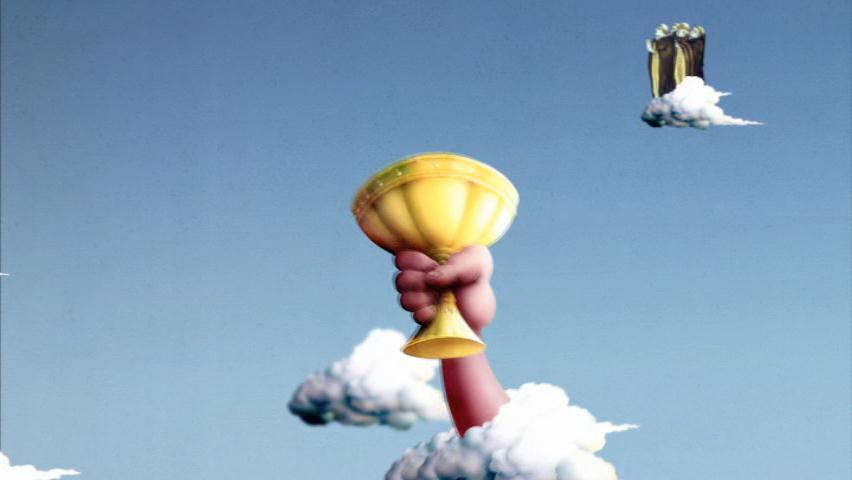
\includegraphics[width=0.8\textwidth]{grail.jpg}
%  \caption[Voorbeeld figuur.]{\label{fig:grail}Voorbeeld van invoegen van een figuur. Zorg altijd voor een uitgebreid bijschrift dat de figuur volledig beschrijft zonder in de tekst te moeten gaan zoeken. Vergeet ook je bronvermelding niet!}
%\end{figure}

%\begin{listing}
%  \begin{minted}{python}
%    import pandas as pd
%    import seaborn as sns

    %penguins = sns.load_dataset('penguins')
    %sns.relplot(data=penguins, x="flipper_length_mm", y="bill_length_mm", hue="species")
  %\end{minted}
  %\caption[Voorbeeld codefragment]{Voorbeeld van het invoegen van een codefragment.}
%\end{listing}

%\lipsum[7-20]

%\begin{table}
%  \centering
%  \begin{tabular}{lcr}
%    \toprule
%    \textbf{Kolom 1} & \textbf{Kolom 2} & \textbf{Kolom 3} \\
%    $\alpha$         & $\beta$          & $\gamma$         \\
%    \midrule
%    A                & 10.230           & a                \\
%    B                & 45.678           & b                \\
%    C                & 99.987           & c                \\
%    \bottomrule
%  \end{tabular}
%  \caption[Voorbeeld tabel]{\label{tab:example}Voorbeeld van een tabel.}
%\end{table}



\section{Digitale onboarding en gebruikersprovisioning}

\subsection{Onboarding binnen organisaties}

Volgens de Cambridge Dictionary wordt onboarding omschreven als ``het proces waarin nieuwe medewerkers vertrouwd raken met hun functie en de organisatie, en met de manier waarop de organisatie functioneert'' (eigen vertaling) \autocite{Cambridge}. Onboarding omvat dus niet uitsluitend administratieve handelingen, maar ook het integreren van nieuwe medewerkers binnen de werking en cultuur van een organisatie.

Volgens \textcite{Studytube2024} kan onboarding beschouwd worden als het proces waarbij nieuwe medewerkers hun functie, collega’s en organisatie leren kennen. Tijdens deze fase maken medewerkers kennis met de interne werking van de organisatie en bouwen zij hun eerste professionele contacten op.

Het doel van onboarding is om nieuwe medewerkers zo snel mogelijk vertrouwd te maken met hun nieuwe werkomgeving zodat zij zelfstandig hun taken kunnen uitvoeren. Daarnaast speelt onboarding ook een belangrijke rol op sociaal vlak. Nieuwe medewerkers die zich snel betrokken voelen bij een organisatie ontwikkelen doorgaans meer motivatie en engagement tegenover hun werkgever. Volgens \textcite{Studytube2024} draagt een gevoel van betrokkenheid bij aan de intrinsieke motivatie van medewerkers om actief bij te dragen aan de organisatie.

Verder benadrukt \textcite{Personio} dat een kwalitatief onboardingproces een positieve invloed heeft op de retentie van medewerkers. Onboarding beperkt zich daarbij niet tot de eerste werkdag, maar vormt een proces dat zich over meerdere weken of maanden kan uitstrekken. De eerste werkdag wordt eerder beschouwd als een oriëntatiefase binnen het bredere onboardingproces.

Binnen moderne organisaties speelt digitale onboarding een steeds belangrijkere rol. Tijdens digitale onboarding krijgen nieuwe medewerkers toegang tot de systemen, applicaties en digitale middelen die noodzakelijk zijn om hun functie uit te oefenen. Dit omvat onder andere gebruikersaccounts, toegangsrechten, e-mailvoorzieningen en toegang tot gedeelde bestanden.

Volgens \textcite{Personioa} verwijst digitale onboarding naar het proces waarbij nieuwe medewerkers ingewerkt worden met behulp van digitale tools en softwareplatformen. Naast technische configuraties omvat dit eveneens digitale communicatie, documentatie en ondersteuning tijdens de integratie van nieuwe medewerkers binnen de organisatie.

Binnen grotere IT-omgevingen wordt digitale onboarding vaak gekoppeld aan identity- en accessmanagementsystemen zodat toegangsbeheer centraal en gecontroleerd beheerd kan worden. Een efficiënte digitale onboarding is belangrijk omdat medewerkers hierdoor sneller operationeel inzetbaar worden. Wanneer noodzakelijke gebruikersaccounts of toegangsrechten niet tijdig beschikbaar zijn, kan dit leiden tot vertragingen, verminderde productiviteit en een minder positieve eerste ervaring binnen de organisatie.

\subsection{Offboarding binnen organisaties}

Volgens \textcite{Acerta} is offboarding net zo belangrijk als onboarding. Offboarding is eigenlijk het tegenovergestelde van onboarding. Het gaat over hoe iemand in een organisatie wordt behandeld bij het uit dienst gaan. Indien offboarding correct gebeurd kan je van een oude werknemer een ambassadeur maken van jouw organisatie \autocite{Acerta}.

Waar onboarding gericht is op de integratie van nieuwe medewerkers, focust offboarding zich op het correcte en respectvolle beëindigen van de arbeidsrelatie. Volgens experts uit de HR-praktijk verdient hierbij niet enkel de juridische afhandeling aandacht, maar ook de ervaring van de vertrekkende medewerker en de impact op het resterende team \autocite{Arens2024}. Niet enkel de ervaring en definitie van offboarding voor een voormalig werknemer is belangrijk. Offboarding kan ook refereren naar alle processen die behoren tot het beëindigen van een professionele relatie \autocite{Detsika2025}. 

Ook van de kant van een werknemer van de ICT-dienst is offboarding belangrijk, binnen organisaties omvat dit onder meer het intrekken van toegangsrechten, het deactiveren van gebruikersaccounts en het terugnemen van bedrijfsmiddelen zoals laptops en badges \autocite{Detsika2025}. Dit is belangrijk aangezien gebruikers die na het eindigen van hun contract, toegang blijven behouden, mogelijk bedrijfsgegevens aan andere bedrijven kunnen geven. Er kunnen dus zowel gegevens van de file server overgenomen worden als ook toegangen tot het netwerk behouden worden.

Een effectief offboardingproces is belangrijk voor zowel organisatorische continuïteit als informatiebeveiliging. Bij het vertrek van medewerkers moeten organisaties niet enkel administratieve en juridische stappen uitvoeren, maar ook toegangsrechten beheren, gebruikersaccounts deactiveren en bedrijfsmiddelen correct innemen. Een gebrekkig offboardingproces kan leiden tot beveiligingsrisico’s en verlies van organisatorische kennis \parencite{Detsika2025}.

\subsection{Manuele versus geautomatiseerde processen}

Binnen veel organisaties verloopt onboarding nog steeds via manuele workflows waarbij verschillende diensten afzonderlijke taken uitvoeren. Bij manuele onboarding moet de IT-dienst gebruikersaccounts, toegangsrechten en mailboxconfiguraties individueel aanmaken en configureren. Daarnaast moeten vaak bijkomende taken uitgevoerd worden, zoals het versturen van welkomstmails of het voorbereiden van toegangsdocumenten \autocite{Ramesh2026}.

Volgens \textcite{Radev2023} leiden dergelijke manuele processen regelmatig tot vertragingen, verhoogde administratieve lasten en fouten bij gegevensoverdracht of toegangsbeheer. Vooral het ontbreken van geïntegreerde systemen vormt hierbij een belangrijk knelpunt. Verschillende diensten zijn afhankelijk van elkaar voor het doorgeven van informatie en het uitvoeren van configuraties, waardoor onboardingprocessen vaak gefragmenteerd verlopen.

Bij manuele onboarding moeten medewerkers van de IT-dienst telkens individueel tussenkomen om nieuwe gebruikers volledig te configureren. Hierdoor bestaat een grotere kans op inconsistenties of menselijke fouten, bijvoorbeeld bij het toekennen van rechten, groepslidmaatschappen of licenties.

Geautomatiseerde onboardingprocessen proberen deze manuele handelingen zoveel mogelijk te beperken door workflows en configuraties automatisch uit te voeren op basis van vooraf gedefinieerde regels. Hierdoor kunnen repetitieve taken sneller en consistenter uitgevoerd worden.

Daarnaast bevestigt \textcite{Vitla2023} dat geautomatiseerde onboardingprocessen bijdragen aan een hogere productiviteit doordat medewerkers vanaf hun eerste werkdag onmiddellijk toegang hebben tot de noodzakelijke digitale middelen. Hierdoor kunnen zowel administratieve diensten als IT-afdelingen efficiënter werken en wordt de kans op configuratiefouten beperkt.

\subsection{Automatische gebruikersprovisioning}

Automatische gebruikersprovisioning vormt vandaag een belangrijk onderdeel van moderne identity- en accessmanagementsystemen. Provisioning verwijst naar het proces waarbij gebruikersaccounts, rechten en toegangen automatisch worden aangemaakt, aangepast en beheerd.

Binnen organisaties omvat provisioning onder andere het aanmaken van gebruikersaccounts, het toekennen van groepslidmaatschappen, het configureren van mailboxen en het voorzien van toegang tot applicaties, gedeelde bestanden en andere digitale middelen.

De nood aan geautomatiseerde provisioningprocessen is de afgelopen jaren sterk toegenomen door de groeiende complexiteit van IT-omgevingen en de toenemende afhankelijkheid van digitale middelen vanaf de eerste werkdag van een medewerker. Volgens \textcite{Okta2025} leidt handmatige provisioning niet alleen tot inefficiëntie, maar vormt deze werkwijze eveneens een belangrijk beveiligingsrisico. Inconsistenties in het aanmaken van accounts en het toekennen van rechten kunnen namelijk leiden tot menselijke fouten en ongecontroleerde toegangsrechten.

Automatische provisioning wordt daarom beschouwd als een belangrijke stap richting veilig en efficiënt identiteitsbeheer. Geautomatiseerde workflows maken het mogelijk om consistente configuraties toe te passen op basis van vooraf gedefinieerde regels en sjablonen. Hierdoor verbeteren zowel de schaalbaarheid als de standaardisatie van gebruikersbeheer binnen organisaties.

\section{Identity and Access Management}

\subsection{Identity and Access Management}

Identity and Access Management (IAM) omvat processen en technologieën die instaan voor het beheren van digitale identiteiten en toegangsrechten binnen organisaties. IAM-systemen ondersteunen organisaties bij het controleren van welke gebruikers toegang krijgen tot bepaalde systemen, applicaties en gegevens.

Het IT-departement van een organisatie heeft manieren nodig om te controleren wat gebruikers kunnen raadplegen \autocite{Microsoft2026}. Hierover gaat het dan over zowel mappen en documenten op de file server, als ook programma's en web toepassingen. Dit moet omdat medewerkers enkel toegang krijgen tot documenten en toepassingen waar zij recht op hebben. Denk ook aan licenties toewijzen aan gebruikers. 

Ook het beheer van toegangen zit hier verder in. Dit houdt de wachtwoord regels in, maar ook de regels op vlak van multi factor authenticatie (MFA) in \autocite{Microsoft2026}. De manier waarop deze geconfigureerd wordt hoort er ook bij. Ook de toegang tot de beschikbare wifi netwerken binnen de organisatie zijn hier onderdeel van. 

\subsection{Identity Lifecycle Management}

Een belangrijk onderdeel van IAM is Identity Lifecycle Management (ILM). Volgens \autocite{OneIdentity2023} omvat ILM het volledige beheer van digitale identiteiten gedurende de volledige levenscyclus van een medewerker. Dit gaat van onboarding en functiewijzigingen tot offboarding en het intrekken van toegangsrechten.

Het gaat dus verder dan enkel de onboarding. IT blijft de gehele tijd dat een werknemer bij een organisatie werkt, bezig met het opvolgen van het account en de gebruiker hiervan. Zonder IT zal de gebruiker zijn werk niet of onvolledig kunnen doen. Denk bijvoorbeeld aan een gebruiker die van dienst of functie veranderd. Zonder dat IT de rechten toevoegt voor de nieuwe dienst of functie, kunnen werknemers hun taken niet uitvoeren. Verder is het verwijderen van de oude rechten ook cruciaal. Dit zodanig dat de gebruiker geen toegang heeft op gegevens die niet meer toegankelijk horen te zijn voor hen. 

ILM-systemen ondersteunen organisaties bij het automatisch toekennen van accounts en rechten bij indiensttreding, het aanpassen van toegangen bij functiewijzigingen en het verwijderen van rechten bij uitdiensttreding. Hierdoor kunnen organisaties gebruikersbeheer consistenter uitvoeren en beveiligingsrisico's beperken \autocite{OneIdentity2023}.

Ook offboarding is een onderdeel van ILM. Offboarding is de laatste stap van een het leven van een gebruikersaccount. Volgens \textcite{Cyberark} kunnen ontevreden werknemers of hackers slapende accounts of verouderde gebruikersrechten misbruiken om aanvallen uit te voeren of vertrouwelijke gegevens te stelen. Dit is uiteraard een groot risico en bevestigd opnieuw waarom ILM belangrijk is.

\subsection{AI binnen IAM-systemen}

Moderne IAM-oplossingen maken steeds vaker gebruik van AI-ondersteunde functionaliteiten. \textcite{Hariharan2025} beschrijft hoe AI-gedreven IAM-systemen risico's kunnen analyseren en automatisch toegangsrechten kunnen voorstellen op basis van functies, gedragspatronen en historische gegevens.

Dergelijke systemen worden voornamelijk toegepast binnen grotere enterprise-omgevingen waar complexe rechtenstructuren aanwezig zijn. Binnen kleinere organisaties en publieke instellingen ligt de focus echter vaker op eenvoudiger automatiseringsprocessen via workflowsystemen, scripts en API-koppelingen.

\subsection{Rolgebaseerde toegangsbeheer}

Role-base access control (RBAC) is het beheer van controles op vlak van rollen. Iedere rol die een gebruiker kan hebben, representeert een nieuwe set van toegangen die aanwezig zijn \autocite{Lindemulder}. Zo zal iemand van de personeelsdienst gegevens kunnen zien over alle medewerkers, maar iemand van vergunningen niet. Ook omgekeerd zullen de medewerkers van vergunningen de gegevens van bijvoorbeeld wegenis kunnen raadplegen, maar werknemers van de personeelsdienst niet. Enkel medewerkers van de IT-dienst kunnen in theorie toegang krijgen tot alle gegevens. Dit is noodzakelijk want anders kunnen gebruikers geen rechten krijgen tot bepaalde mappen. 

Op basis van de rollen, worden er groepen opgesteld binnen de systemen voor rechten. Denk bij Windows aan Active Directory. Deze groepen krijgen dan één of meerdere rollen toegewezen. In deze groepen worden dan, afhankelijk of er een volledige dienst toegang hiertoe moet hebben, andere groepen of gebruikers toegevoegd. 

In een ideale situatie, worden er per functie groepen opgesteld met daarop allemaal rechten. In de praktijk werkt dit helaas niet altijd zo. Vaak worden rechten nog toegekend aan gebruikers in plaats van aan groepen. Hierdoor wordt het principe van RBAC niet correct toegepast. 

Er moet altijd gewerkt worden met het principe om zo minimaal mogelijke rechten te hebben. Hoe meer rechten een gebruiker heeft, hoe groter het risico bij die gebruiker is. Wanneer iemand rechten niet nodig heeft, dienen deze ook meteen verwijderd te worden. 

\section{Workflowautomatisering}

\subsection{Automatisering van bedrijfsprocessen}

Workflowautomatisering verwijst naar het automatiseren van repetitieve processen en taken binnen organisaties. Door workflows te automatiseren kunnen organisaties manuele handelingen beperken, foutenmarges verkleinen en processen efficiënter uitvoeren.

Binnen IT-omgevingen wordt workflowautomatisering onder andere gebruikt voor gebruikersbeheer, toegangscontrole, gegevensverwerking en systeemintegraties. De opkomst van low-code en no-code platformen heeft ervoor gezorgd dat dergelijke automatiseringen toegankelijker zijn geworden voor organisaties zonder uitgebreide softwareontwikkelingsafdelingen.

\subsection{Low-code en no-code platformen}

Low-code en no-code platformen maken het mogelijk om workflows te ontwikkelen via grafische interfaces en vooraf gebouwde componenten. Hierdoor kunnen processen sneller ontwikkeld en aangepast worden zonder uitgebreide programmeerkennis.

Het grote voordeel van dit soort platformen, is dat gebruikers zelf aan de slag kunnen met automatiseren, zonder de nodige IT kennis te hebben \autocite{Carlson2026}. Hierdoor is de nodige IT support voor gelijkaardige projecten, in een wereld zonder low-code en no-code platformen, overbodig. In essentie is het aan de slag gaan met programmeren, zonder het programmeren. Er wordt gebruik gemaakt van bouwstenen waar achterliggend code achter zit.

Er zijn uiteraard ook beperkingen. Zo kan je enkel de bouwstenen gebruiken die reeds geconfigureerd zijn. Wanneer er een taak is waarvoor deze nog niet bestaat, moet er toch weer geschakeld worden naar programmeren waar IT support opnieuw voor nodig is.

Voor eenvoudige projecten, is dit zeker een optie die kan bekeken worden. Voor complexere configuraties in projecten, kan er ook gebruikt van gemaakt worden, is samenwerking met programmerende oplossingen. 

Volgens \textcite{Nwibe2026} behoren Activepieces, Zapier en Make tot de meest gebruikte alternatieven voor Microsoft Power Automate binnen workflowautomatisering. Elk platform beschikt over specifieke eigenschappen, integratiemogelijkheden en beperkingen.

\section{Workflowautomatiseringstools}

\subsection{Microsoft Power Automate}

Microsoft Power Automate is een workflowplatform binnen het Microsoft-ecosysteem dat gebruikt wordt voor het automatiseren van processen tussen cloud- en on-premisesomgevingen. Het platform ondersteunt integraties met Microsoft 365, SharePoint, Teams, Forms en diverse externe applicaties.

Volgens \autocite{Microsoft2024} kan Power Automate gebruikt worden voor het automatisch verwerken van gegevens afkomstig uit Microsoft Forms en Excel. Daarnaast ondersteunt het platform het uitvoeren van scripts en het aanroepen van externe systemen via connectors en API-koppelingen.

Verder beschrijft \textcite{Microsoft2021} dat er integraties bestaan tussen Power Automate en PowerShell, waardoor automatiseringsprocessen gecombineerd kunnen worden met systeembeheer en Active Directory-functionaliteiten.

\subsection{Zapier}

Zapier is een cloudgebaseerd automatiseringsplatform dat integraties aanbiedt tussen een groot aantal online diensten en applicaties. Het platform richt zich voornamelijk op eenvoudige workflowautomatisering via vooraf gedefinieerde connectors.

Hoewel Zapier ondersteuning biedt voor scripting via onder andere JavaScript en Python, beschikt het platform niet over een ingebouwde PowerShell-integratie. Integraties met PowerShell verlopen daarom doorgaans via API-aanroepen of externe systemen.

\subsection{Make}

Make is een visueel workflowplatform dat organisaties toelaat om complexe automatiseringsprocessen op te bouwen via een grafische interface. Het platform ondersteunt uitgebreide API-integraties en conditionele workflows.

Net zoals Zapier beschikt Make niet over een directe ingebouwde PowerShell-module. Integratie met PowerShell vereist daarom bijkomende configuraties of externe tussenlagen.

\subsection{Activepieces}

Activepieces is een open-source automatiseringsplatform dat zich richt op flexibele workflowautomatisering en integraties tussen cloudtoepassingen. Het platform ondersteunt verschillende connectors en uitbreidingen via API-koppelingen.

Volgens de officiële documentatie beschikt Activepieces momenteel niet over een directe integratie met PowerShell, waardoor bijkomende configuratie noodzakelijk kan zijn voor systeembeheer binnen Windows-omgevingen.

\subsection{n8n}

n8n is een open-source workflowplatform dat organisaties toelaat om workflows lokaal of in de cloud te hosten. Het platform onderscheidt zich door zijn uitbreidbaarheid en uitgebreide ondersteuning voor API-integraties.

Daarnaast biedt n8n ondersteuning voor scripting en technische configuraties via JSON-verwerking en aangepaste modules. Hierdoor biedt het platform meer flexibiliteit, maar vereist het doorgaans ook meer technische expertise voor implementatie en onderhoud.

\subsection{Vergelijking van workflowplatformen}

Workflowplatformen verschillen onderling op vlak van integratiemogelijkheden, gebruiksgemak, schaalbaarheid, prijsmodellen en ondersteuning voor scripting. Sommige platformen richten zich voornamelijk op cloudintegraties en gebruiksvriendelijke interfaces, terwijl andere oplossingen meer flexibiliteit bieden via open-source-functionaliteiten en technische configuratiemogelijkheden.

Bij de selectie van een workflowplatform spelen factoren zoals beveiliging, compatibiliteit met bestaande infrastructuur, ondersteuning voor PowerShell en integratie met hybride IT-omgevingen een belangrijke rol.

\section{PowerShell en Active Directory}

\subsection{PowerShell binnen systeembeheer}

PowerShell wordt binnen Windows-omgevingen veel gebruikt voor systeembeheer en automatisering. Via scripts kunnen beheerders repetitieve taken automatiseren en configuraties centraal beheren.

Binnen identity- en accessmanagement wordt PowerShell vaak toegepast voor het beheren van gebruikersaccounts, groepsrechten en directorystructuren.

\subsection{De cmdlet New-ADUser}

De PowerShell-cmdlet New-ADUser maakt deel uit van de Active Directory-module en wordt gebruikt om nieuwe gebruikersobjecten aan te maken binnen een domeinomgeving \autocite{Microsoft2024a}.

Deze cmdlet ondersteunt uitgebreide configuratiemogelijkheden, waaronder het instellen van gebruikersattributen zoals accountnamen, wachtwoorden, organisatorische eenheden en groepslidmaatschappen. Hierdoor kunnen organisaties consistente gebruikersaccounts implementeren binnen een Active Directory-omgeving.

Verder benadrukt \textcite{Microsoft2024a} dat New-ADUser frequent wordt toegepast binnen scripts en automatiseringsprocessen voor onboarding en gebruikersbeheer. Door parameters en standaardconfiguraties te combineren kunnen beheerders efficiënter werken en menselijke fouten beperken.

\section{Hybride IT-omgevingen}

\subsection{Cloud- en on-premisesomgevingen}

Veel organisaties maken vandaag gebruik van hybride IT-omgevingen waarbij bepaalde systemen in de cloud draaien terwijl andere toepassingen lokaal on-premises blijven functioneren. Deze aanpak combineert de schaalbaarheid en flexibiliteit van cloudplatformen met de controle en gegevensbescherming van lokale infrastructuren.

Volgens \textcite{Ahuja2024} kiezen organisaties vaak voor hybride infrastructuren om privacygevoelige gegevens lokaal te bewaren terwijl andere diensten via cloudplatformen worden aangeboden.

\subsection{Microsoft On-Premises Data Gateway}

Binnen hybride Microsoft-omgevingen wordt de On-Premises Data Gateway gebruikt om veilige verbindingen mogelijk te maken tussen cloudtoepassingen en lokale systemen \autocite{Microsoft2025}.

Deze gateway maakt het mogelijk om gegevens en workflows vanuit cloudplatformen zoals Microsoft Power Automate of Microsoft Forms te koppelen aan lokale systemen zoals Active Directory of lokale databanken.

\section{Wetgeving en gegevensbescherming}

\subsection{GDPR binnen gebruikersbeheer}

Bij onboardingprocessen worden persoonsgegevens verwerkt zoals namen, contactgegevens, functietitels en gebruikersrechten. Organisaties dienen daarom rekening te houden met de Europese General Data Protection Regulation (GDPR).

De GDPR legt organisaties verplichtingen op rond gegevensbescherming, toegangscontrole en veilige verwerking van persoonsgegevens. Binnen gebruikersbeheer betekent dit onder andere dat toegangsrechten beperkt moeten blijven tot noodzakelijke systemen en dat persoonsgegevens beveiligd verwerkt moeten worden.

\subsection{Toegangscontrole en compliance}

Naast gegevensbescherming speelt ook compliance een belangrijke rol binnen identity- en accessmanagement. Organisaties moeten kunnen aantonen welke gebruikers toegang hebben tot bepaalde systemen en op welke manier toegangsrechten worden beheerd.

Automatisering kan hierbij bijdragen aan consistente toegangscontrole, logging en standaardisatie van processen. Hierdoor kunnen organisaties beter voldoen aan beveiligingsrichtlijnen en auditvereisten.

\section{Onderzoekskloof}

Wat opvalt binnen de bestaande literatuur is dat veel onderzoeken zich voornamelijk richten op enterprise-omgevingen en grootschalige IAM-platformen. Studies die specifiek focussen op kleinere overheidsinstanties of gemeentelijke IT-omgevingen zijn eerder beperkt.

Daarnaast behandelen veel onderzoeken algemene onboardingprocessen zonder specifiek in te gaan op de integratie tussen personeelsgegevens, workflowautomatisering en Active Directory binnen publieke organisaties.

Er bestaat bijgevolg nog een beperkte hoeveelheid praktijkgerichte literatuur rond geautomatiseerde gebruikersprovisioning binnen gemeentelijke IT-omgevingen. Deze bachelorproef wil bijdragen aan dit domein door te onderzoeken hoe een geautomatiseerd onboardingproces gerealiseerd kan worden binnen een hybride infrastructuur met aandacht voor workflowautomatisering, Active Directory-integratie en gegevensbescherming.

%%=============================================================================
%% Methodologie
%%=============================================================================

\chapter{\IfLanguageName{dutch}{Methodologie}{Methodology}}%
\label{ch:methodologie}

%% TODO: In dit hoofstuk geef je een korte toelichting over hoe je te werk bent
%% gegaan. Verdeel je onderzoek in grote fasen, en licht in elke fase toe wat
%% de doelstelling was, welke deliverables daar uit gekomen zijn, en welke
%% onderzoeksmethoden je daarbij toegepast hebt. Verantwoord waarom je
%% op deze manier te werk gegaan bent.
%% 
%% Voorbeelden van zulke fasen zijn: literatuurstudie, opstellen van een
%% requirements-analyse, opstellen long-list (bij vergelijkende studie),
%% selectie van geschikte tools (bij vergelijkende studie, "short-list"),
%% opzetten testopstelling/PoC, uitvoeren testen en verzamelen
%% van resultaten, analyse van resultaten, ...
%%
%% !!!!! LET OP !!!!!
%%
%% Het is uitdrukkelijk NIET de bedoeling dat je het grootste deel van de corpus
%% van je bachelorproef in dit hoofstuk verwerkt! Dit hoofdstuk is eerder een
%% kort overzicht van je plan van aanpak.
%%
%% Maak voor elke fase (behalve het literatuuronderzoek) een NIEUW HOOFDSTUK aan
%% en geef het een gepaste titel.

In de eerste fase van het onderzoek is een analyse uitgevoerd van het huidige onboarding- en off\-boar\-ding\-pro\-ces\-sen binnen het lokale gemeentebestuur van Berlare. Deze analyse is noodzakelijk om inzicht te verkrijgen in welke stappen momenteel worden toegepast binnen de processen en hoeveel tijd deze stappen in beslag nemen. Hiervoor zijn gesprekken gevoerd met betrokken medewerkers om na te gaan welke taken zij uitvoeren en welke systemen daarbij gebruikt worden.

Daarnaast is in deze fase onderzocht welke fouten zich het vaakst voordoen en waar knelpunten optreden binnen het bestaande proces. Op basis van deze bevindingen is een lijst met requirements opgesteld, die geordend is volgens functionaliteit en prioriteit. Deze fase heeft de basis gevormd voor het verdere onderzoek en is afgerond tijdens de tweede week van februari. \newline

In de tweede fase is een literatuurstudie uitgevoerd. Het doel van deze studie is het in kaart brengen van bestaande technologieën, systemen en methodieken die ingezet worden voor de automatisatie van onboardingprocessen. Door het bestuderen van relevante literatuur en bestaande oplossingen is er inzicht verkregen in mogelijke technische benaderingen die toepasbaar zijn binnen de context van een lokaal bestuur. 
Op basis van deze studie is een selectie gemaakt van systemen en technologieën die potentieel een positieve invloed kunnen hebben op het onboardingproces. Deze fase is deels afgerond tegen het einde van februari. Deels omdat dit een fase is die tijdens het verder uitwerken van de proof of concept, steeds opnieuw is gedaan. Bij het vastlopen van het uitwerken, is er uiteraard opnieuw onderzocht. \newline

De derde en meest omvangrijke fase van het onderzoek heeft bestaan uit het uitwerken van een proof of concept. In deze fase zijn de resultaten uit de analyse- en literatuurfase gecombineerd om een zo realistisch en toepasbaar mogelijke oplossing te ontwerpen en te implementeren. Het doel van dit proof of concept was aan te tonen hoe een geautomatiseerd onboarding- en offboardingproces kan functioneren binnen de bestaande IT-infrastructuur van de gemeente Berlare.

Er wordt hierbij gebruik gemaakt van API-koppelingen, die door Power Automate zelf verwerkt worden, waarbij gegevens vanuit Microsoft Forms gekoppeld worden aan verschillende attributen binnen Active Directory. Daarnaast zijn automatisatie- en orkestratietools, Microsoft Power Automate, ingezet om de robuustheid en schaalbaarheid van de oplossing te verhogen. \newline

Na de implementatie van het proof of concept is een evaluatiefase gevolgd. In deze fase is het ontwikkelde systeem geëvalueerd aan de hand van de eerder opgestelde requirements. Daarbij is nagegaan in welke mate het proof of concept voldoet aan de vooropgestelde functionele en technische verwachtingen. Daarnaast is een vergelijking gemaakt tussen de bestaande processen en de geautomatiseerde oplossing, met bijzondere aandacht voor tijdsbesparing, foutreductie en gebruiksgemak. Waar mogelijk is feedback van betrokken medewerkers meegenomen om sterktes en verbeterpunten van de oplossing te identificeren. \newline

Hoewel de verschillende fasen chronologisch zijn voorgesteld, zijn ze iteratief doorlopen. Inzichten die voortkomen uit de proof-of-concept- en evaluatiefase hebben aanleiding gegeven tot een aanvullend literatuuronderzoek of bijkomende bevragingen bij medewerkers. Deze iteratieve aanpak draagt bij aan een eindresultaat dat realistisch, toepasbaar en technisch onderbouwd is.\newline

Figuur \ref{fig:Methodologie} toont een eenvoudige versie van de methodologie.

\begin{figure}[htbp]
    \centering
    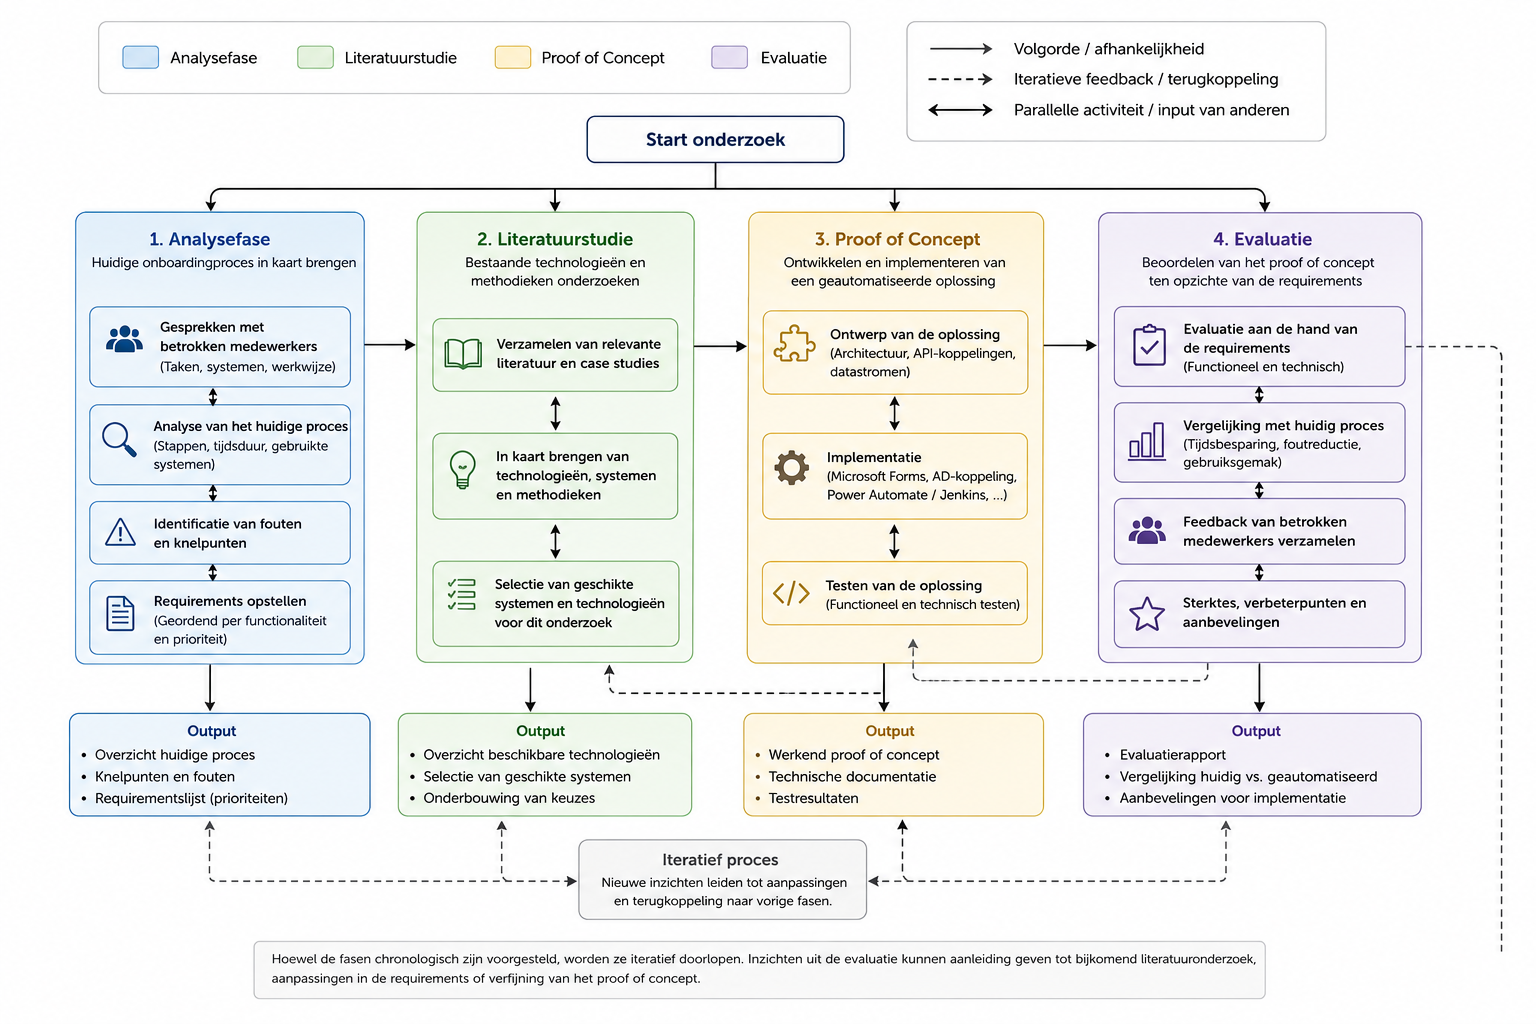
\includegraphics[width=1\textwidth]{Methodologie.png}
    \caption[Methodologie]{Visuele voorstelling van de methodologie}
    \label{fig:Methodologie}
\end{figure}


% Voeg hier je eigen hoofdstukken toe die de ``corpus'' van je bachelorproef
% vormen. De structuur en titels hangen af van je eigen onderzoek. Je kan bv.
% elke fase in je onderzoek in een apart hoofdstuk bespreken.

%%
%%Huidig onboardingsproces
%%

\chapter{Huidige onboarding- en offboardingprocessen}
\label{ch:HuidigeProcessen}

In dit hoofdstuk wordt de huidige werkwijze besproken die gebruikt wordt binnen het gemeentebestuur van Berlare.

\section{Beschrijving van de huidige processen}

De beschrijving van de huidige processen binnen de gemeente Berlare.

\subsection{Huidig onboardingsproces}

Het huidige onboardingsproces binnen het gemeentebestuur van Berlare omvat verschillende administratieve en technische stappen om de toegang van een nieuwe medewerker tot interne systemen op te bouwen.

\subsubsection{Algemene werking}

Het bestaande onboardingproces van nieuwe medewerkers binnen het gemeentebestuur werd geanalyseerd om de huidige werkwijze, betrokken diensten en uitgevoerde stappen in kaart te brengen.

Het proces omvat administratieve, technische en communicatieve handelingen die voornamelijk door de personeelsdienst en de ICT-dienst worden uitgevoerd. De personeelsdienst verzamelt de noodzakelijke persoonsgegevens en functiegegevens en bezorgt deze aan de ICT-dienst, die vervolgens de benodigde accounts en toegangen configureert.

Figuur~\ref{fig:HuidigeOnboarding} geeft een vereenvoudigd overzicht van de huidige onboardingflow binnen het gemeentebestuur.

\begin{figure}[!h]
    \centering
    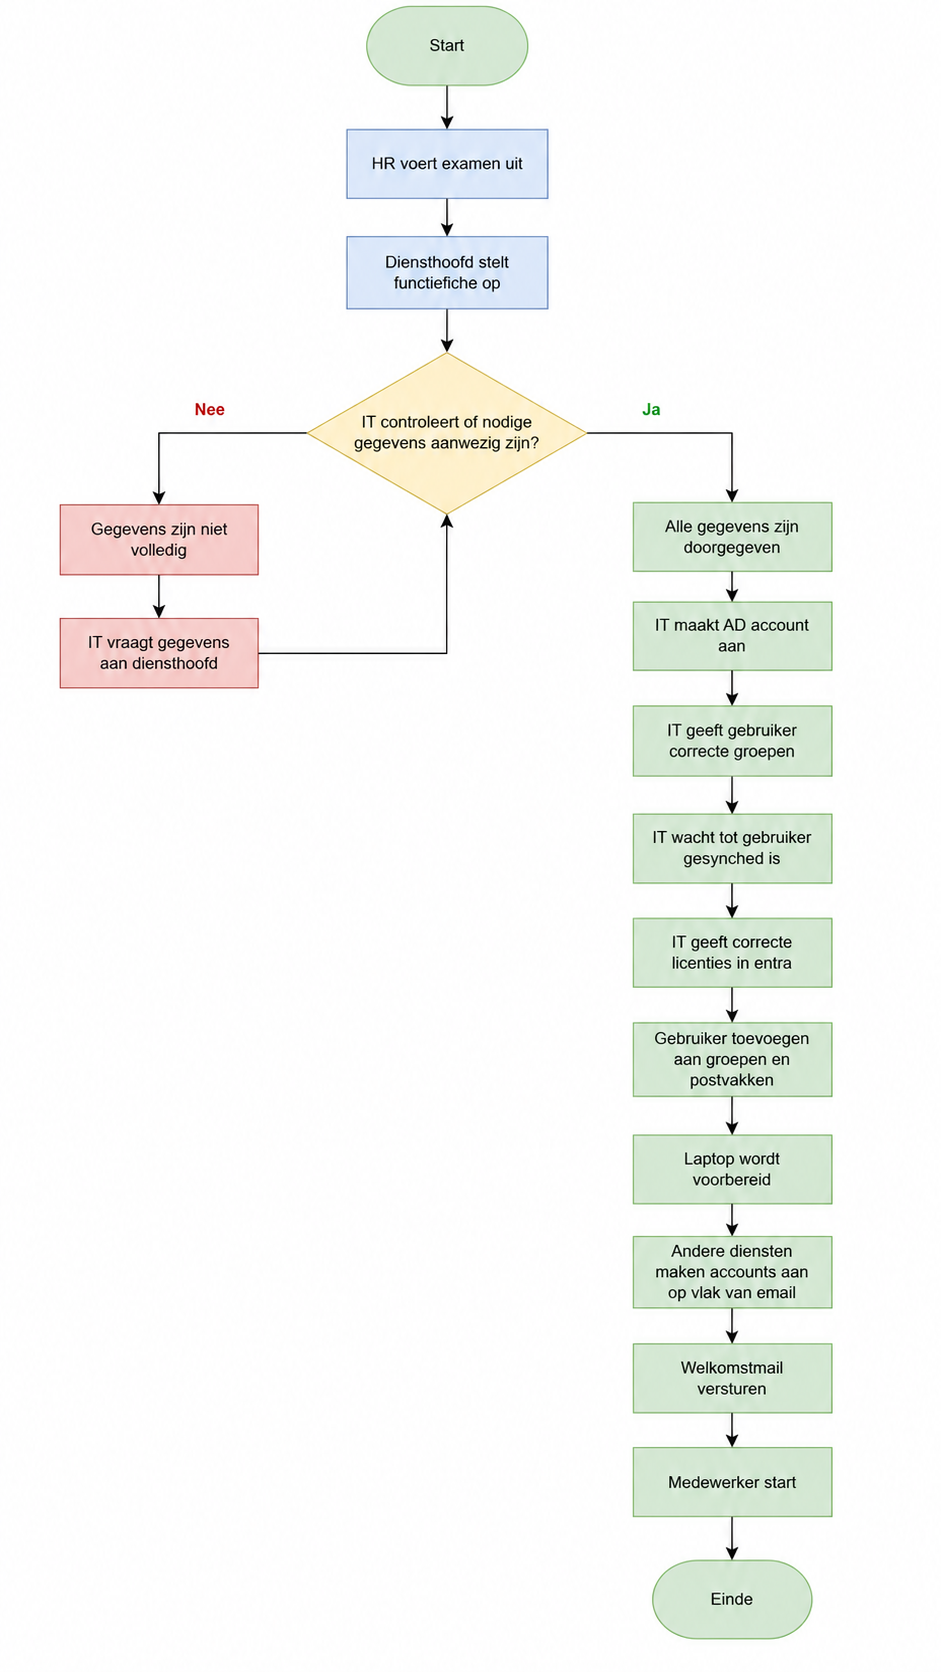
\includegraphics[width=0.75\textwidth]{HuidigeOnboarding.png}
    \caption[Huidig onboardingsproces]{Overzicht van het huidige onboardingproces en de interactie tussen de betrokken diensten}
    \label{fig:HuidigeOnboarding}
\end{figure}

\subsubsection{Huidige werkwijze binnen de ICT-dienst}

Binnen de ICT-dienst verloopt een groot deel van het onboardingproces momenteel manueel. Gebruikersaccounts worden individueel aangemaakt binnen Active Directory, waarna gebruikers handmatig toegevoegd worden aan relevante beveiligingsgroepen en distributielijsten.

Daarnaast worden mailboxen geconfigureerd en worden rechten ingesteld voor verschillende interne systemen en gedeelde mappen. Ook licenties worden afzonderlijk toegekend afhankelijk van de functie en de benodigde softwaretoegang van de medewerker.

Ook de communicatie met de nieuwe medewerker gebeurt grotendeels manueel. Welkomstmails met handleidingen en documentatie worden afzonderlijk verzonden. Daarnaast wordt een tijdelijke wachtwoordbrief gegenereerd, afgedrukt en fysiek bezorgd.

\subsubsection{Fysieke configuratiehandelingen}

Naast digitale configuraties omvat het onboardingproces eveneens verschillende fysieke handelingen binnen de ICT-dienst. Hierbij gaat het onder andere om het voorbereiden van hardware, het installeren van toestellen en het configureren van softwarepakketten.

Deze handelingen worden momenteel individueel uitgevoerd afhankelijk van de functie en de noden van de nieuwe medewerker. Hierdoor bestaat het onboardingproces uit een combinatie van digitale configuraties en fysieke installatietaken.

\subsection{Huidig offboardingsproces}

Het huidige offboardingsproces binnen het gemeentebestuur van Berlare omvat verschillende administratieve en technische stappen om de toegang van een vertrekkende medewerker tot interne systemen af te bouwen.

\subsubsection{Algemene werking}

De personeelsdienst of het diensthoofd meldt de uitdiensttreding aan de ICT-dienst. Vervolgens worden verschillende configuraties handmatig aangepast, waaronder het uitschakelen van gebruikersaccounts, verwijderen van toegangsrechten en aanpassen van gedeelde postvakken.

Omdat deze handelingen afhankelijk zijn van de einddatum van het contract, worden ze doorgaans op of kort na de laatste werkdag uitgevoerd

Figuur \ref{fig:HuidigeOffboarding} toont een visuele voorstelling van het huidige offboardingsproces.

\begin{figure}[!h]
    \centering
    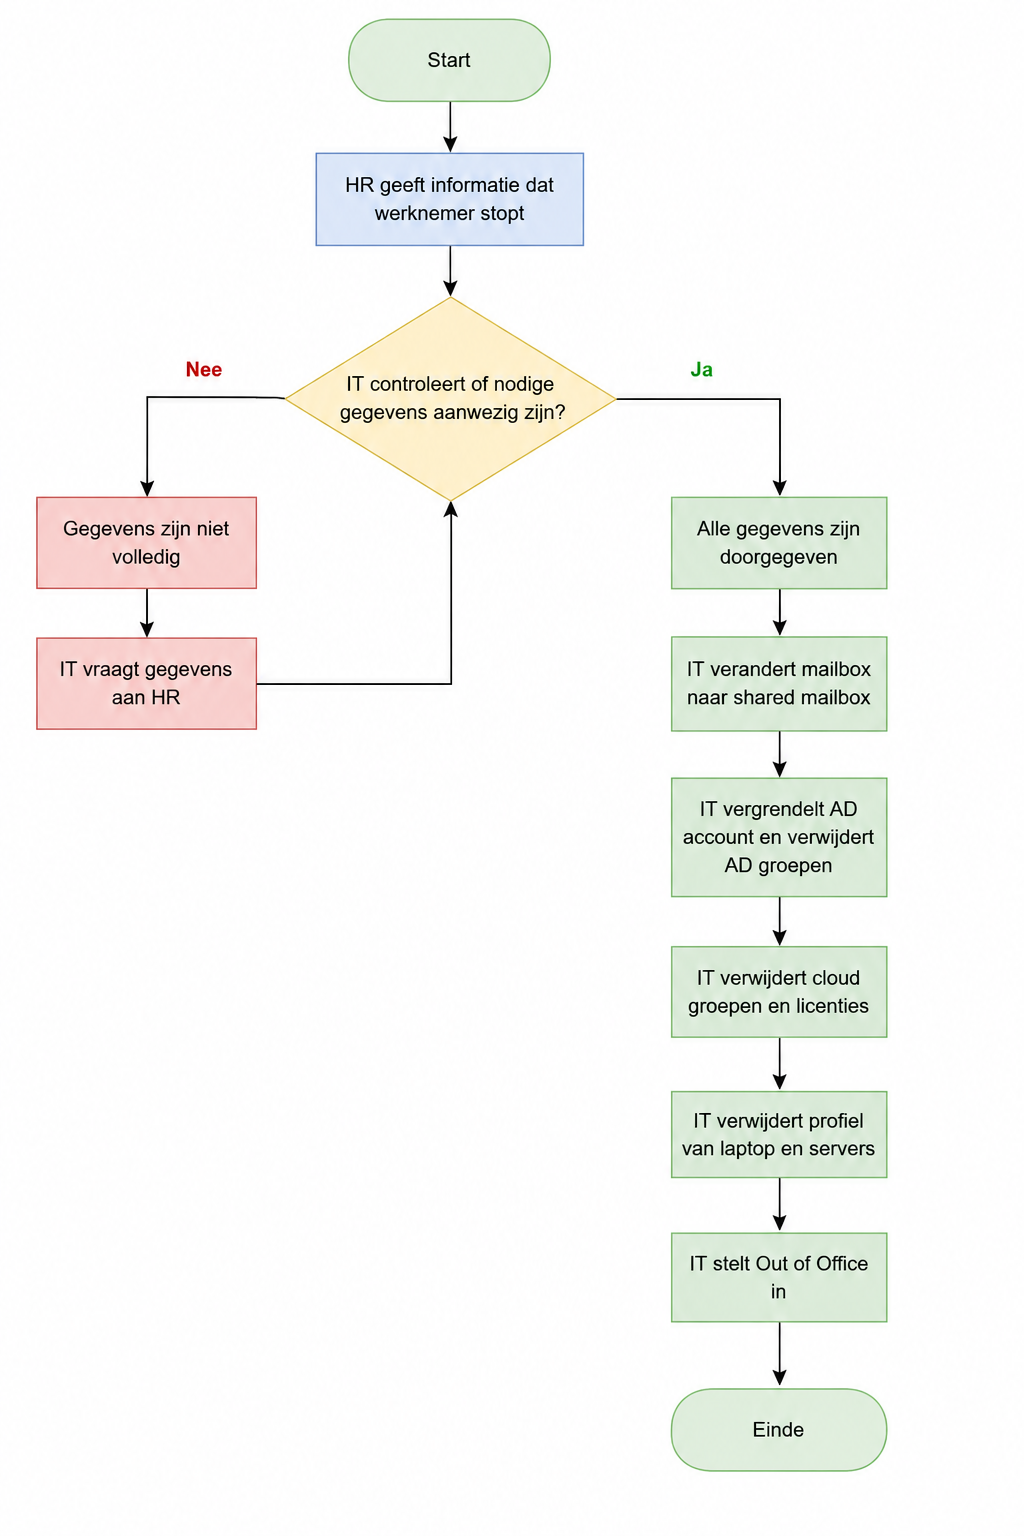
\includegraphics[width=0.75\textwidth]{HuidigeOffboarding.png}
    \caption[Huidig offboardingsproces]{Overzicht van het huidige offboardingproces}
    \label{fig:HuidigeOffboarding}
\end{figure}

\subsubsection{Werkwijze binnen de ICT-dienst}

Binnen de ICT-dienst verloopt het offboardingproces momenteel grotendeels manueel. Medewerkers moeten handmatig gebruikersaccounts opzoeken binnen Active Directory en deze vervolgens uitschakelen of aanpassen. Daarnaast worden gebruikers verwijderd uit beveiligingsgroepen, distributielijsten en Microsoft 365-groepen. Ook mailboxrechten op gedeelde postvakken moeten afzonderlijk verwijderd worden.

De mailbox van een voormalige medewerker wordt omgezet naar een gedeeld postvak zodat historische communicatie behouden blijft. Daarnaast wordt een Out of Office ingesteld met informatie over de opvolging van de mailbox. Ook de toegekende Microsoft 365-licenties worden verwijderd zodat deze opnieuw beschikbaar zijn.

Verder moeten van de laptops de gebruikersaccounts verwijderd worden. Ook op de servers moeten deze opnieuw verwijderd worden. Op deze manier verdwijnen de bestanden die lokaal op laptops opgeslagen waren, waardoor er dus ruimte vrij komt op een laptop en deze dus opnieuw gebruikt kan worden. 

\subsubsection{Beheer van toegangen en mailboxen}

Een belangrijk onderdeel van het offboardingproces bestaat uit het correct verwijderen van toegangsrechten. Wanneer accounts of rechten niet tijdig verwijderd worden, bestaat het risico dat voormalige medewerkers nog toegang behouden tot interne systemen of gevoelige gegevens.

Omdat toegangsrechten verspreid beheerd worden over verschillende platformen, waaronder Active Directory, Entra ID en Exchange Online, vereist dit proces momenteel meerdere afzonderlijke handelingen binnen verschillende beheertools.

Daarnaast bestaat er momenteel geen centrale opvolging waarmee eenvoudig gecontroleerd kan worden welke onderdelen van het offboardingproces reeds uitgevoerd werden.

\section{Communicatie en samenwerking tussen diensten}

Voor de hudige processen binnen het gemeentebestuur van Berlare is er ook samenwerking en communicatie nodig tussen de interne diensten.

\subsection{Afhankelijkheden tussen diensten}

Binnen het huidige onboardingproces zijn meerdere diensten afhankelijk van elkaar om bepaalde stappen correct te kunnen uitvoeren. De personeelsdienst levert de noodzakelijke gegevens aan voor het aanmaken of uitschakelen van gebruikersaccounts, terwijl andere interne diensten afhankelijk zijn van het beschikbaar zijn van een e-mailadres of gebruikersaccount om toegang te voorzien tot dienstspecifieke toepassingen.

Hierdoor ontstaat een proces waarbij verschillende stappen pas uitgevoerd kunnen worden nadat voorgaande configuraties succesvol voltooid zijn. Een correcte communicatie tussen diensten speelt daarom een belangrijke rol binnen het onboardingproces.

\subsection{Terugkoppeling van uitgevoerde taken}

Binnen de huidige processen gebeurt de terugkoppeling van uitgevoerde taken voornamelijk manueel. Medewerkers communiceren onderling wanneer bepaalde configuraties of administratieve stappen voltooid zijn.

Andere diensten zijn afhankelijk van meldingen of terugkoppelingen wanneer gebruikersaccounts succesvol aangemaakt werden. Deze informatie is noodzakelijk om bijkomende configuraties uit te voeren binnen dienstspecifieke softwaretoepassingen.

Deze werkwijze maakt het moeilijker om de voortgang van het onboardingproces centraal op te volgen en kan leiden tot onduidelijkheid over de status van bepaalde stappen.

\section{Knelpunten binnen de huidige processen}

Binnen het gemeentebestuur van Berlare zijn er een aantal duidelijke knelpunten binnen beide processen.

\subsection{Manuele configuraties}

Een groot deel van het onboarding- en offboardingproces wordt momenteel manueel uitgevoerd. Het aanmaken en uitschakelen van gebruikersaccounts, het beheren van groepslidmaatschappen en licenties en het configureren van mailboxen vereisen verschillende repetitieve handelingen van de ICT-dienst.

Daarnaast verhoogt manuele configuratie de kans op inconsistenties en menselijke fouten. Foutieve groepslidmaatschappen, ontbrekende rechten of vergeten configuraties kunnen leiden tot bijkomende correcties en vertragingen. Verder kan het niet verwijderen van gebruikers doordat dit vergeten wordt, leiden tot veiligheidsrisico's.

\subsection{Gebrek aan centrale opvolging}

Een bijkomend knelpunt is het ontbreken van een centrale opvolging van uitgevoerde taken. Omdat verschillende stappen verspreid uitgevoerd worden door meerdere medewerkers en diensten, ontstaat er soms onduidelijkheid over de voortgang van het proces. Hierdoor ontstaan afhankelijkheden waarbij medewerkers moeten navragen of bepaalde configuraties reeds voltooid zijn.

\subsection{Complexiteit van onboarding en offboarding}

Beide processen bestaan uit verschillende onderling verbonden stappen waarbij meerdere systemen betrokken zijn. Naast gebruikersbeheer in Active Directory moeten eveneens mailboxen, licenties, distributielijsten en interne toepassingen correct geconfigureerd of aangepast worden.

Daarnaast verhoogt de hybride infrastructuur, waarbij zowel Active Directory als Microsoft 365 en Entra ID gebruikt worden, de complexiteit van beide processen. Synchronisaties tussen lokale en cloudomgevingen zorgen ervoor dat bepaalde configuraties pas uitgevoerd kunnen worden nadat eerdere stappen succesvol voltooid werden.

Deze combinatie van afhankelijkheden, verschillende beheersystemen en manuele configuraties bemoeilijkt een efficiënte opvolging van onboarding en offboarding binnen de huidige werking van het gemeentebestuur.

%%
%%Analyse en ontwerp van de oplossing
%%

\chapter{Analyse en ontwerp van de oplossing}
\label{ch:analyseontwerp}

\section{Doelstellingen van de oplossing}

Op basis van de analyse van het huidige onboarding- en offboardingsprocedures werd vastgesteld dat verschillende stappen binnen de ICT-dienst repetitief en manueel uitgevoerd worden. Hierdoor neemt het verwerken van nieuwe medewerkers relatief veel tijd in beslag en ontstaat een verhoogde kans op menselijke fouten. Daarnaast zijn verschillende diensten afhankelijk van elkaar voor het uitvoeren van bepaalde configuraties, waardoor vertragingen kunnen ontstaan wanneer terugkoppelingen ontbreken.

Het doel van dit onderzoek is daarom het ontwerpen van een oplossing die een deel van het onboarding- en van het offboardingsproces automatiseert binnen de bestaande ICT-omgeving van het gemeentebestuur van Berlare. De focus ligt hierbij voornamelijk op het automatisch verwerken van gebruikersgegevens en het automatisch aanmaken of uitschakelen van gebruikersaccounts binnen de Active Directory-omgeving.

Daarnaast moet de oplossing zorgen voor een betere opvolging van uitgevoerde taken en een efficiëntere samenwerking tussen verschillende diensten binnen het onboarding- en offboardingsproces. Het uiteindelijke doel is om de administratieve belasting te verminderen, de foutmarge te verkleinen en de doorlooptijd van beide processen te beperken.

\section{Requirements van de oplossing}

\subsection{Functionele requirements}

\subsubsection{Must-have requirements}

De belangrijkste doelstelling van deze bachelorproef is het ontwikkelen van een geautomatiseerd systeem waarbij gebruikersaccounts automatisch aangemaakt worden op basis van gegevens die aangeleverd worden door de personeelsdienst.

De focus ligt hierbij voornamelijk op het automatisch aanmaken van gebruikersaccounts binnen Active Directory, het instellen van relevante attributen binnen de lokale infrastructuur, het toekennen van Microsoft 365-licenties en het automatisch voorzien van basisrechten afhankelijk van de dienst van de medewerker.

Daarnaast moet de oplossing voorzien in een vorm van terugkoppeling zodat de status van uitgevoerde onboardings beschikbaar is voor andere betrokken diensten binnen de organisatie.

\subsubsection{Should-have requirements}

Naast de basisfunctionaliteiten zijn er verschillende uitbreidingen die bij voorkeur aanwezig zijn binnen de oplossing. Hieronder vallen onder andere het automatisch toekennen van rechten op gedeelde postvakken en het automatisch toevoegen van gebruikers aan distributielijsten binnen Microsoft 365.

Deze functionaliteiten verhogen de gebruiksvriendelijkheid van het systeem en verminderen bijkomende manuele configuraties binnen de ICT-dienst.

\subsubsection{Could-have requirements}

Binnen deze categorie vallen functionaliteiten die een meerwaarde bieden, maar niet noodzakelijk zijn voor de basiswerking van de oplossing.

Een eerste uitbreiding is het automatisch versturen van een welkomstmail naar nieuwe medewerkers met praktische informatie en handleidingen. Daarnaast behoort ook het automatiseren van het offboardingproces tot deze categorie.

Hoewel offboarding een belangrijk onderdeel vormt van identiteits- en toegangsbeheer binnen organisaties, lag de primaire focus van deze bachelorproef op onboarding. Indien mogelijk werd echter ook een gedeeltelijke automatisering van offboarding opgenomen binnen de oplossing.

\subsubsection{Would-have requirements}

De laatste categorie omvat uitbreidingen die wenselijk zijn, maar momenteel moeilijk realiseerbaar zijn binnen de bestaande infrastructuur.

Hieronder valt het volledig automatiseren van rechtenbeheer op de file server. Binnen de huidige omgeving bestaat een complexe rechtenstructuur waarbij bepaalde toegangen historisch rechtstreeks aan individuele gebruikers toegewezen werden in plaats van via veiligheidsgroepen.

Door deze inconsistente structuur is het momenteel niet mogelijk om alle rechten volledig automatisch en betrouwbaar toe te wijzen. Een volledige herstructurering van de bestaande rechtenomgeving zou hiervoor noodzakelijk zijn.

\subsection{Niet-functionele requirements}

De oplossing moet compatibel zijn met de bestaande hybride infrastructuur van het gemeentebestuur van Berlare. Zowel lokale on-premisesystemen als cloudtoepassingen binnen Microsoft 365 moeten ondersteund worden.

Daarnaast moet de oplossing veilig functioneren binnen de bestaande infrastructuur. Enkel bevoegde medewerkers mogen toegang hebben tot de automatiseringsflows en gevoelige configuraties.

Verder moet de oplossing voldoende flexibel en onderhoudbaar zijn zodat toekomstige uitbreidingen en aanpassingen mogelijk blijven.

\section{Analyse van automatiseerbare processen}

\subsection{Automatiseerbare taken}

Binnen het huidige onboardingproces werden verschillende taken geïdentificeerd die zich lenen tot automatisering. Het gaat hierbij voornamelijk om digitale configuraties die volgens vaste patronen uitgevoerd worden binnen de ICT-omgeving.

Een eerste belangrijke taak is het automatisch aanmaken van gebruikersaccounts binnen Active Directory. Momenteel gebeurt dit handmatig waarbij gebruikersgegevens individueel ingevoerd worden. Daarnaast worden gebruikers eveneens manueel toegevoegd aan beveiligingsgroepen en distributielijsten.

Ook het toekennen van licenties binnen Entra ID gebeurt momenteel afzonderlijk per gebruiker. Omdat deze toewijzingen grotendeels gebaseerd zijn op functie en dienst, kan dit proces geautomatiseerd worden door gebruikers automatisch aan de correcte groepen toe te voegen.

Verder werden ook terugkerende communicatieve taken geïdentificeerd. Zo kunnen meldingen of terugkoppelingen automatisch verstuurd worden wanneer bepaalde configuraties succesvol uitgevoerd werden. Hierdoor kunnen andere diensten sneller verder werken met hun eigen configuraties.

Naast onboarding werden ook verschillende onderdelen van het offboardingproces geïdentificeerd die zich lenen tot automatisering. Wanneer een medewerker de organisatie verlaat, moeten verschillende toegangen en configuraties aangepast of verwijderd worden binnen zowel Active Directory als Microsoft 365.

Momenteel gebeurt dit grotendeels manueel door de ICT-dienst. Hierbij worden gebruikersaccounts gedeactiveerd, groepslidmaatschappen verwijderd, mailboxrechten aangepast en licenties ingetrokken. Omdat deze stappen volgens vaste procedures verlopen, kunnen ook deze processen gedeeltelijk geautomatiseerd worden.

Daarnaast is offboarding vanuit beveiligingsoogpunt een belangrijk proces. Het tijdig verwijderen van toegangsrechten vermindert het risico op ongewenste toegang tot interne systemen en gegevens nadat een medewerker uit dienst gegaan is.


\subsection{Niet-automatiseerbare taken}

Niet alle onderdelen van het onboardingproces lenen zich tot automatisering. Bepaalde taken vereisen fysieke tussenkomst of individuele beoordeling door medewerkers van de ICT-dienst.

Zo gebeurt het selecteren van geschikte hardware momenteel op basis van de functie en de specifieke noden van de medewerker. Daarnaast vereisen ook de installatie van toestellen, het aansluiten van randapparatuur en bepaalde softwareconfiguraties manuele handelingen.

Ook het fysiek verwerken van documenten, zoals het afdrukken en overhandigen van tijdelijke wachtwoorden, valt buiten de scope van dit onderzoek. Hiervoor zouden bijkomende gespecialiseerde systemen noodzakelijk zijn.

De focus van dit onderzoek ligt daarom voornamelijk op het automatiseren van digitale configuraties en identiteitsbeheer binnen de bestaande IT-omgeving.

Ook binnen het offboardingproces blijven bepaalde taken afhankelijk van fysieke tussenkomst door de ICT-dienst. Zo kunnen het ophalen van hardware, het fysiek controleren van toestellen en het volledig herinstalleren van laptops niet automatisch uitgevoerd worden binnen de scope van deze oplossing.


\section{Technische vereisten}

Binnen de bestaande infrastructuur van het gemeentebestuur wordt gebruikgemaakt van een hybride omgeving waarbij zowel cloudtoepassingen als lokale on-premisesystemen aanwezig zijn. Hierdoor moet de oplossing kunnen communiceren met beide omgevingen.

De gebruikersaccounts worden lokaal beheerd binnen Active Directory, terwijl bepaalde cloudtoepassingen gebruikmaken van Entra ID. Hierdoor moet de oplossing rekening houden met synchronisatie tussen beide platformen.

Daarnaast vormt compatibiliteit met bestaande Microsoft-diensten een belangrijke vereiste binnen het project. Binnen de organisatie wordt reeds gebruikgemaakt van Microsoft Power Automate, Microsoft 365 en PowerShell-gebaseerde beheertools. Hierdoor moet de oplossing integreren met deze bestaande infrastructuur.

Verder moet de oplossing voldoende flexibel zijn om rekening te houden met verschillende diensten, sites en organisatorische structuren binnen de Active Directory-omgeving.

Daarnaast moet de oplossing voldoende veilig functioneren binnen de bestaande infrastructuur. Omdat gevoelige configuraties uitgevoerd worden binnen zowel Active Directory als Microsoft 365, moet toegangsbeheer correct afgeschermd worden en mogen enkel bevoegde medewerkers de automatiseringsflows kunnen uitvoeren.

\section{Keuze van technologieën}

Binnen het onderzoek werden verschillende automatiseringsplatformen onderzocht die gebruikt kunnen worden voor workflowautomatisering en systeemintegratie.

Platformen zoals Zapier, Make en Activepieces bieden mogelijkheden voor cloudgebaseerde automatisering en integratie tussen verschillende toepassingen. Deze platformen richten zich voornamelijk op algemene workflowautomatisering tussen cloudservices.

Binnen dit project vormde ondersteuning voor lokale PowerShell-uitvoering echter een belangrijke vereiste. Omdat gebruikersaccounts lokaal binnen Active Directory aangemaakt moeten worden, moet de oplossing kunnen communiceren met on-premisesystemen.

Daarnaast werd binnen de organisatie reeds gebruikgemaakt van infrastructuur gebaseerd op Microsoft en bestaande automatiseringsprojecten binnen Power Automate. Hierdoor bood Power Automate belangrijke voordelen op vlak van compatibiliteit en integratie met bestaande Microsoft-diensten.

Verder ondersteunt Power Automate de combinatie van cloudflows en lokale desktopflows via Power Automate Desktop en Machine Runtime, waardoor communicatie met lokale systemen mogelijk wordt binnen een hybride omgeving.

Op basis van deze vereisten werd gekozen om de verdere implementatie uit te werken met Microsoft Power Automate in combinatie met PowerShell-gebaseerde automatisering.

Daarnaast moet de oplossing niet alleen nieuwe accounts kunnen aanmaken, maar ook bestaande gebruikersaccounts veilig kunnen aanpassen of deactiveren tijdens het offboardingproces. Hiervoor moet eveneens communicatie mogelijk zijn met Exchange Online voor het beheren van mailboxrechten, distributiegroepen en gedeelde postvakken.

\section{Ontwerp van de oplossing}
\subsection{Algemene oplossing}

De ontworpen oplossing bestaat uit verschillende componenten die samenwerken binnen zowel de cloudomgeving als de lokale infrastructuur van de gemeente.

De invoer van gebruikersgegevens gebeurt via Microsoft Forms. Wanneer een nieuwe aanvraag wordt verzonden, worden de gegevens verwerkt binnen een cloudflow in Power Automate. Deze flow verwerkt de ontvangen gegevens en bereidt deze voor op verdere verwerking binnen de lokale omgeving.

Omdat Active Directory lokaal beheerd wordt, moet de cloudomgeving kunnen communiceren met een on-premisesysteem. Hiervoor wordt gebruikgemaakt van Power Automate Desktop en Power Automate Machine Runtime. Deze componenten vormen de brug tussen de cloudflow en de lokale serveromgeving.

Binnen de lokale omgeving wordt een PowerShell-script uitgevoerd dat verantwoordelijk is voor het aanmaken of uitschakelen van gebruikersaccounts, het toewijzen of verwijderen van groepen en het configureren van verschillende Active Directory-attributen.

Bij onboarding moet eerst gewacht worden tot de synchronisatie tussen Active Directory en Entra ID voltooid is voordat cloudconfiguraties uitgevoerd kunnen worden. Bij offboarding is deze synchronisatie minder kritisch omdat het uitschakelen van accounts voornamelijk lokaal verwerkt wordt en de blokkering van cloudtoegang automatisch volgt via synchronisatie.

Nadien worden de distributielijsten en gedeelde postvakken toegevoegd of verwijderd bij de gebruiker. ODe configuratie van distributielijsten en gedeelde postvakken gebeurt via PowerShell-scripts die communiceren met Exchange Online. Hiervoor werd gekozen omdat Power Automate momenteel geen volwaardige connectoren aanbiedt voor het beheren van mailboxrechten binnen Exchange Online.

Als laatste stap binnen het configuratieproces wordt automatisch een welkomstmail verzonden naar de nieuwe medewerker. Deze mail bevat verschillende handleidingen en praktische informatie die noodzakelijk zijn om vlot van start te kunnen gaan tijdens de eerste werkdag. Hierbij kan gedacht worden aan informatie over het verbinden met het draadloze netwerk, het gebruik van printers en andere interne ICT-toepassingen.

Na het voltooien van alle configuratiestappen wordt een terugkoppeling uitgevoerd binnen het opvolgsysteem. Omdat het algemene opvolgingssysteem van een parallel project momenteel nog in ontwikkeling is, werd tijdelijk gekozen voor een tussenoplossing op basis van Excel. Hierbij wordt de status van de verwerking automatisch aangepast binnen hetzelfde Excelbestand dat tijdens de testfase gebruikt werd. Op deze manier kan eenvoudig gecontroleerd worden of de volledige flow succesvol werd uitgevoerd en de gebruiker correct werd aangemaakt.

Figuur~\ref{fig:ArchitectuurOnboarding} toont een vereenvoudigd overzicht van de algemene architectuur van de oplossing voor onboarding.

\begin{figure}[htbp]
    \centering
    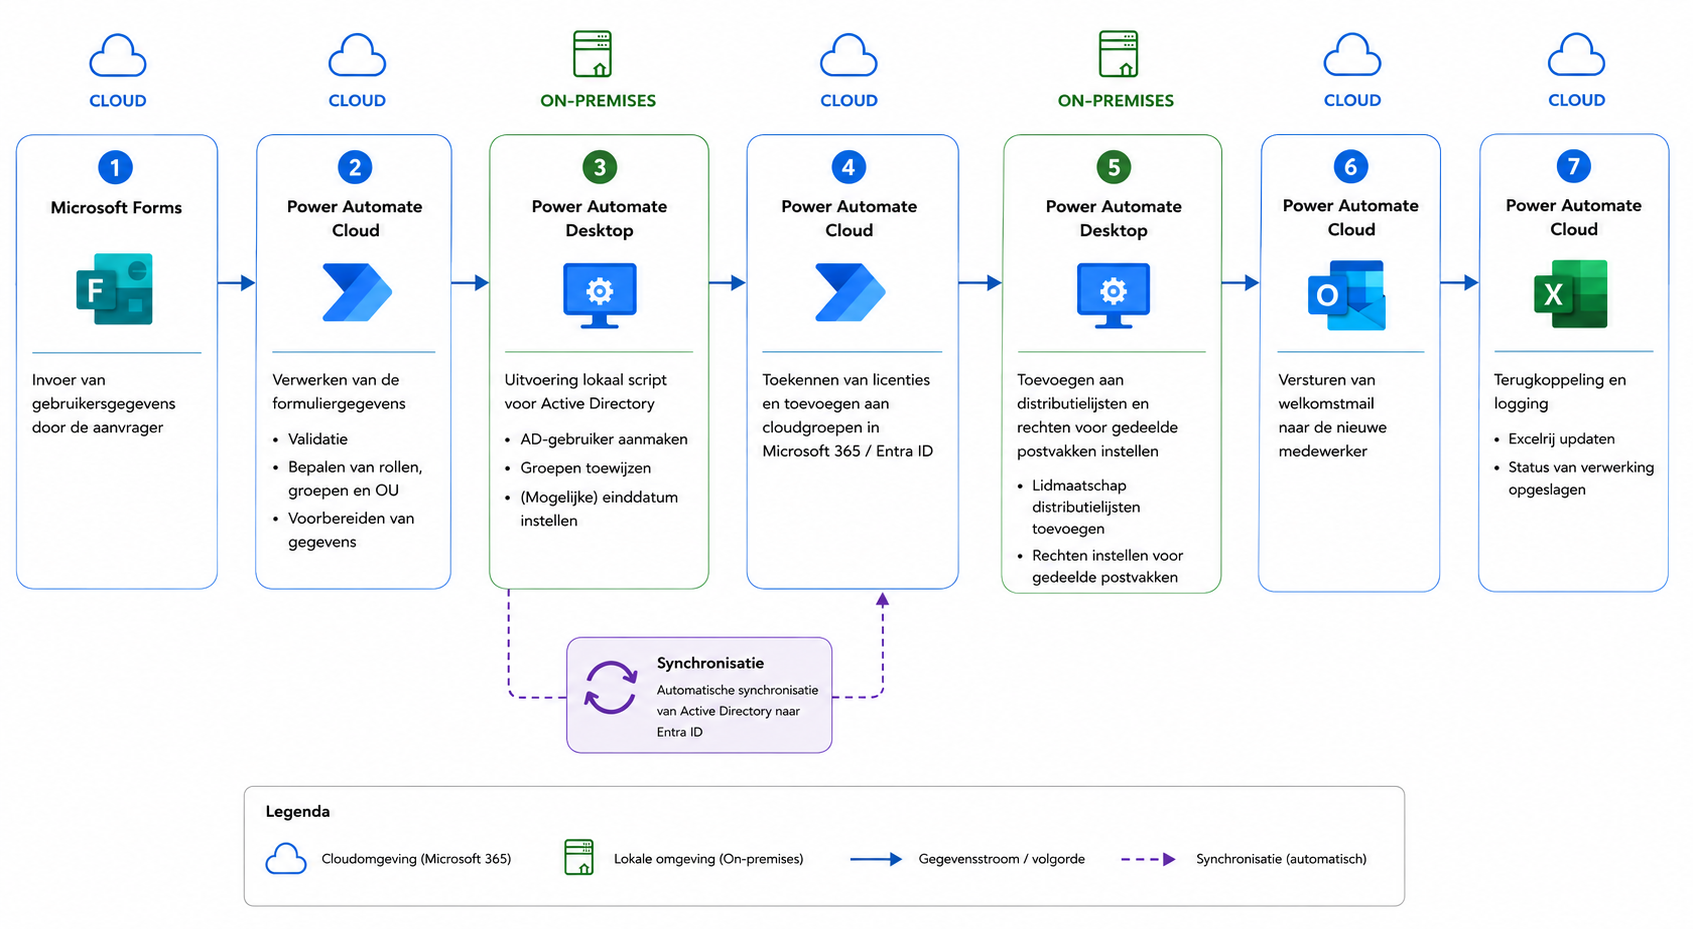
\includegraphics[width=1\textwidth]{Architectuur.png}
    \caption[Power Automate flow]{Vereenvoudigde voorstelling van de Power Automate Flow voor onboarding}
    \label{fig:ArchitectuurOnboarding}
\end{figure}

\subsection{Ontwerp van de onboardingsflow}

De automatiseringsflow werd ontworpen op basis van de bestaande onboardingprocedure binnen de ICT-dienst. Hierbij werd een verwerking voorzien waarbij gebruikersgegevens automatisch vertaald worden naar configuraties binnen Active Directory en Entra ID.

Binnen Microsoft Forms worden verschillende gegevens verzameld, waaronder voornaam, achternaam, functietitel, dienst, site, telefoonnummer en contractinformatie. Deze gegevens worden vervolgens verwerkt binnen Power Automate.

Omdat bepaalde vragen binnen het formulier afhankelijk zijn van eerder gekozen antwoorden, moet de flow rekening houden met dynamische gegevensstructuren. Hiervoor worden conditionele controles gebruikt om de correcte diensten en bijhorende OU-structuren te bepalen.

Daarnaast moet de oplossing rekening houden met verschillen tussen cloud- en on-premisesystemen. Hierdoor werd gekozen voor een architectuur waarbij de cloudflow verantwoordelijk is voor gegevensverwerking en orchestration, terwijl lokale PowerShell-scripts instaan voor de configuratie van Active Directory.

\subsection{Ontwerp van de offboardingflow}

Naast het automatiseren van onboarding werd eveneens een geautomatiseerde offboardingflow ontworpen. Deze flow heeft als doel om gebruikersaccounts en toegangsrechten automatisch af te bouwen wanneer een medewerker uit dienst gaat.

De offboarding start vanuit een afzonderlijk Microsoft Forms-formulier waarin de personeelsdienst de gegevens van de medewerker invoert, waaronder het e-mailadres, de einddatum van het contract en de reden van uitdiensttreding.

Omdat gebruikers pas gedeactiveerd mogen worden nadat de laatste werkdag verstreken is, werd een wachmechanisme voorzien binnen de cloudflow van Power Automate. De flow blijft actief totdat de opgegeven einddatum bereikt werd.

Na het bereiken van deze datum wordt automatisch een desktopflow gestart die verschillende PowerShell-scripts uitvoert binnen zowel Exchange Online als Active Directory. Hierbij wordt de mailbox van de gebruiker omgezet naar een gedeeld postvak, worden mailboxrechten verwijderd, groepslidmaatschappen aangepast en wordt het Active Directory-account gedeactiveerd.

Daarnaast worden Microsoft 365-groepen en licenties automatisch verwijderd zodat ongebruikte cloudlicenties opnieuw beschikbaar worden binnen de organisatie.

Door deze automatisering wordt het offboardingproces consistenter uitgevoerd en wordt het risico verminderd dat voormalige medewerkers nog toegang behouden tot interne systemen of gegevens.

\subsection{OU-structuur binnen Active Directory}

Binnen de Active Directory-omgeving van de gemeente wordt gebruikgemaakt van een hiërarchische structuur van Organizational Units (OU's). Gebruikers worden hierbij ondergebracht op basis van site en dienst.

Afhankelijk van de organisatorische structuur kunnen diensten zich op verschillende niveaus binnen de directorystructuur bevinden. Sommige sites bevatten afzonderlijke OU's per dienst, terwijl andere diensten gezamenlijk ondergebracht worden binnen één gedeelde OU.

Zo bevat de site ``Gemeentehuis'' afzonderlijke OU's voor diensten zoals personeelsdienst, vergunningen en informatica. Andere locaties, zoals de onthaalpoort aan het Donkmeer, groeperen meerdere diensten binnen dezelfde OU omdat deze organisatorisch nauwer samenwerken.

Door deze variatie binnen de directorystructuur moet de automatiseringsoplossing rekening houden met verschillende mappings tussen diensten en hun overeenkomstige OU-locaties.

Figuur~\ref{fig:OrganizationalUnit} toont een vereenvoudigd overzicht van de gebruikte OU-structuur binnen Active Directory.

\clearpage

\begin{figure}[htbp]
    \centering
    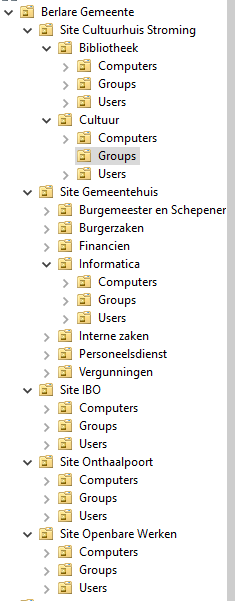
\includegraphics[width=0.4\textwidth]{OrganizationalUnit.png}
    \caption[OU structuur]{Vereenvoudigde voorstelling van de OU-structuur binnen de Active Directory-omgeving van de gemeente.}
    \label{fig:OrganizationalUnit}
\end{figure}

\subsection{Synchronisatie tussen Active Directory en Entra ID}

Binnen de hybride omgeving van de gemeente worden gebruikersaccounts eerst lokaal aangemaakt binnen Active Directory. Vervolgens worden deze accounts automatisch gesynchroniseerd naar Entra ID.

Deze synchronisatie gebeurt echter niet onmiddellijk maar volgens vaste synchronisatiecycli. Hierdoor ontstaat een vertraging tussen het aanmaken van een gebruiker binnen Active Directory en de beschikbaarheid van deze gebruiker binnen Entra ID.

Omdat bepaalde cloudconfiguraties, zoals licentietoewijzingen, pas uitgevoerd kunnen worden nadat de gebruiker beschikbaar is binnen Entra ID, moet de automatiseringsflow rekening houden met deze wachttijd.

Hiervoor werd een controlemechanisme ontworpen waarbij periodiek gecontroleerd wordt of de gebruiker reeds beschikbaar is binnen Entra ID. Pas wanneer de synchronisatie succesvol voltooid werd, kunnen bijkomende cloudconfiguraties uitgevoerd worden.

Ook tijdens offboarding blijft deze synchronisatie belangrijk zodat wijzigingen aan gebruikersaccounts en groepslidmaatschappen correct doorstromen naar de cloudomgeving.

\section{Testomgeving en validatieaanpak}

Tijdens de eerste ontwikkelingsfase was nog geen volledige productieomgeving beschikbaar voor het uitvoeren van geautomatiseerde cloudflows. Daarnaast vereisen bepaalde onderdelen van Power Automate bijkomende licenties.

Om de ontwikkeling toch te kunnen opstarten, werd eerst gewerkt met een testomgeving waarbij gebruikersgegevens vanuit een Excelbestand verwerkt werden. De kolommen binnen dit bestand werden opgesteld volgens dezelfde structuur als de uiteindelijke variabelen binnen Power Automate.

Deze aanpak maakte het mogelijk om de PowerShell-scripts afzonderlijk te ontwikkelen en te testen zonder afhankelijk te zijn van de volledige cloudomgeving. Daarnaast kon hierdoor gecontroleerd worden of gebruikers correct aangemaakt werden en de juiste groepslidmaatschappen ontvingen.

De tijdelijke testomgeving vormde hierdoor een belangrijke tussenfase binnen het ontwikkelingsproces van de uiteindelijke oplossing.




%%
%%Implementatie van de oplossing
%%

\chapter{Implementatie van de oplossing}
\label{ch:ImplementatieVanDeOplossing}

\section{Verwerking van invoergegevens}

De automatiseringsflow start met het verzamelen van gegevens via een Microsoft Forms-formulier met de naam ``Onboarding''. Dit formulier wordt gebruikt door de personeelsdienst om de noodzakelijke gegevens van nieuwe medewerkers centraal aan te leveren aan de ICT-dienst.

Binnen het formulier worden verschillende gegevens opgevraagd die noodzakelijk zijn voor het uitvoeren van de onboarding. Hierbij gaat het onder andere om de voornaam, achternaam, startdatum, eventuele einddatum van het contract, functietitel, telefoonnummer, site en dienst van de medewerker. Daarnaast kunnen ook bijkomende configuraties meegegeven worden, zoals de gedeelde postvakken waarvoor toegang vereist is en de distributielijsten waaraan de gebruiker toegevoegd moet worden.

Om de kans op foutieve invoer te beperken, werd een extra controleveld toegevoegd waarbij bevestigd moet worden dat de ingevoerde gegevens nagekeken werden. Op deze manier wordt geprobeerd om de kwaliteit van de brongegevens zo hoog mogelijk te houden voordat de automatische verwerking start.

De toegang tot het formulier is beperkt via de beveiligingsinstellingen van Microsoft Forms. Enkel medewerkers van de personeelsdienst en de ICT-dienst kunnen het formulier invullen. In de praktijk wordt het formulier hoofdzakelijk gebruikt door de personeelsdienst, terwijl de ICT-dienst toegang behoudt voor testdoeleinden en voor het opnieuw uitvoeren van een onboardingproces wanneer een fout optreedt.

\section{Cloudflow binnen Power Automate}

Na het verzenden van het Microsoft Forms-formulier wordt automatisch een cloudflow binnen Microsoft Power Automate gestart. Deze flow vormt de centrale verwerkingslaag van de oplossing en staat in voor het ophalen, verwerken en voorbereiden van de ingevoerde gegevens.

De flow start met de trigger ``Wanneer er een nieuwe reactie wordt verzonden''. Deze trigger detecteert automatisch wanneer een nieuwe onboardingaanvraag werd ingediend via Microsoft Forms. Hierbij wordt het juiste formulier geselecteerd op basis van het unieke formulier-id.

Nadat de flow gestart werd, worden de details van de ingevulde aanvraag opgehaald via de stap ``Reactiedetails ophalen''. Deze stap maakt het mogelijk om alle ingevoerde waarden uit het formulier beschikbaar te maken binnen de flow. De verschillende antwoorden kunnen vervolgens gebruikt worden als dynamische variabelen binnen verdere stappen van het automatiseringsproces.

Omdat bepaalde velden binnen het formulier afhankelijk zijn van eerder gekozen antwoorden, moet de flow rekening houden met conditionele logica. Zo worden bepaalde diensten enkel weergegeven wanneer een specifieke site geselecteerd werd. Hierdoor verschillen de beschikbare invoervelden afhankelijk van de gekozen locatie.

Om deze gegevens uniform te kunnen verwerken binnen de verdere automatisering, worden ``Compose''-stappen gebruikt. Deze stappen zorgen ervoor dat de correcte dienst automatisch geselecteerd wordt op basis van de gekozen site binnen het formulier.

Codefragment ~\ref{lst:ComposeDepartement} vereenvoudigde expressie toont de gebruikte logica.

\begin{lstlisting}[
    caption={Samenstelling van de departementen},
    label={lst:ComposeDepartement}]
    if(site == "Gemeentehuis",
        dienst_gemeentehuis,
        if(site == "Onthaalpoort",
            dienst_onthaalpoort,
            if(site == "Cultuurhuis Stroming",
                dienst_cultuurhuis,
                andere_dienst)))
\end{lstlisting}

Door gebruik te maken van deze conditionele verwerking kan de flow steeds de correcte dienst ophalen, ongeacht welke site geselecteerd werd binnen het formulier. Deze waarden worden later gebruikt voor het bepalen van de correcte OU-structuur en groepsconfiguraties binnen Active Directory.

Naast het bepalen van de dienst wordt binnen de flow eveneens een rolcode samengesteld op basis van het departement van de gebruiker. Deze rolcodes worden later gebruikt binnen de PowerShell-scripts voor het toekennen van groepen, rechten en bijkomende configuraties.

Hiervoor wordt opnieuw gebruikgemaakt van een ``Compose''-stap waarin conditionele logica toegepast wordt. Afhankelijk van het gekozen departement wordt een specifieke rolcode toegekend.

Codefragment ~\ref{lst:ComposeRole} vereenvoudigde expressie toont een voorbeeld van deze verwerking.

\begin{lstlisting}[
    caption={Samenstelling van de rollen},
    label={lst:ComposeRole}]
    if(departement == "Informatica",
        "IT-user",
        if(departement == "Personeelsdienst",
            "HR-user",
            if(departement == "Financien",
                "FI-user",
                "user")))
\end{lstlisting}

\inputminted{powershell}{PowerAutomate.ps1}

Door gebruik te maken van gestandaardiseerde rolcodes kan de verdere verwerking binnen PowerShell en Active Directory eenvoudiger en consistenter verlopen. Daarnaast maakt deze aanpak het mogelijk om rechten en groepslidmaatschappen centraal te beheren op basis van functie of dienst.

Binnen de flow worden daarnaast verschillende variabelen samengesteld die later gebruikt worden binnen de PowerShell-scripts. Hierbij gaat het onder andere om de naam van de gebruiker, de dienst, de organisatorische eenheid binnen Active Directory en bijkomende configuraties zoals distributielijsten of gedeelde postvakken.

Tijdens de eerste ontwikkelingsfase werd gebruikgemaakt van een tijdelijke tussenstap waarbij de gegevens eerst naar een Excelbestand geschreven werden. Deze aanpak maakte het mogelijk om de verwerking van gegevens eenvoudig te controleren voordat de effectieve automatisering binnen Active Directory werd uitgevoerd.

Figuur ~\ref{fig:VoorbeeldOutput} toont voorbeeldoutput die gebruikt werd om te valideren dat de gegevens correct verwerkt werden.

\begin{figure}[htbp]
    \centering
    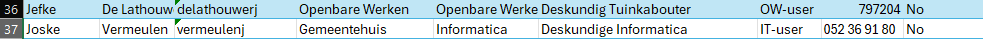
\includegraphics[width=1\textwidth]{Voorbeeldoutput.png}
    \caption[Voorbeeld output Power Automate]{Voorbeeld van de tijdelijke output van de Power Automate flow}
    \label{fig:VoorbeeldOutput}
\end{figure}

Figuur ~\ref{fig:Cloudflow_deel1} toont het eerste deel van de cloudflow binnen Microsoft Power Automate.

\begin{figure}[htbp]
    \centering
    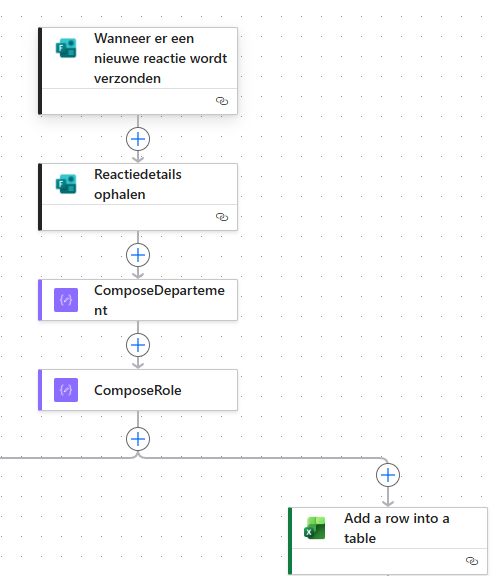
\includegraphics[width=0.9\textwidth]{Cloudflow_deel1.png}
    \caption[Cloudflow binnen Power Automate]{Overzicht van het eerste deel van de cloudflow binnen Microsoft Power Automate.}
    \label{fig:Cloudflow_deel1}
\end{figure}

\section{Desktopflow en PowerShell-integratie}

Omdat Active Directory lokaal beheerd wordt binnen de infrastructuur van het gemeentebestuur, volstaat een gewone cloudflow binnen Microsoft Power Automate niet om gebruikersaccounts rechtstreeks aan te maken of aan te passen. De gebruikers dienen lokaal aangemaakt te worden aangezien er sprake is van een hybride omgeving. Hiervoor is communicatie nodig met de lokale serveromgeving waarop Active Directory beschikbaar is. 

Om deze communicatie mogelijk te maken, wordt gebruikgemaakt van Power Automate Desktop in combinatie met Power Automate Machine Runtime. Deze componenten vormen de verbinding tussen de cloudomgeving van Microsoft Power Automate en de lokale infrastructuur van de gemeente. Power Automate Desktop zal de scripts uitvoeren in een lokale flow en Power Automate Runtime zorgt voor de connectie tussen Power Automate Cloud en Power Automate Desktop. 

Wanneer de cloudflow alle gegevens verwerkt heeft, wordt automatisch een desktopflow gestart op de lokale server. Hierbij worden verschillende parameters doorgestuurd, waaronder de naam van de gebruiker, de dienst, de gekozen site, de rolcode en eventuele bijkomende configuraties zoals distributielijsten of gedeelde postvakken.

\subsection{Automatisch aanmaken en instellen van Active Directory-ge\-brui\-kers}

Binnen de desktopflow wordt een PowerShell-script uitgevoerd dat verantwoordelijk is voor het automatisch aanmaken en configureren van nieuwe gebruikersaccounts binnen Active Directory. Het script ontvangt verschillende parameters vanuit Power Automate, waaronder de voornaam, achternaam, dienst, site, functietitel en rolcode van de gebruiker.

Op basis van deze gegevens worden automatisch de correcte accountgegevens samengesteld, de juiste Organizational Unit bepaald en de noodzakelijke groepslidmaatschappen toegekend.

Codefragment ~\ref{lst:Parameters} toont de parameters die vanuit de desktopflow doorgestuurd worden naar het PowerShell-script.

\begin{lstlisting}[language=PowerShell,
    caption={Parameters},
    label={lst:Parameters}]
    param(
    [string]$FirstName,
    [string]$LastName,
    [string]$Department,
    [string]$Site,
    [string]$Role,
    [string]$Telephone,
    [string]$Title
    )
\end{lstlisting}

Door gebruik te maken van parameters kan hetzelfde script hergebruikt worden voor verschillende gebruikers en diensten zonder manuele aanpassingen aan de code.

\subsubsection{Verwerking van invoergegevens}

Voor het aanmaken van een account worden de ontvangen gegevens eerst gevalideerd en genormaliseerd. Speciale tekens en niet-alfabetische karakters worden verwijderd om problemen met accountnamen en e-mailadressen te vermijden. Door de tekst eerst te normaliseren, worden speciale tekens opgesplitst zodat deze eenvoudiger verwijderd kunnen worden.

Dezelfde verwerking wordt toegepast op zowel de voornaam als de achternaam van de gebruiker.

\begin{lstlisting}[language=PowerShell,
    caption={Aanpassen naam},
    label={lst:AanpassenNaam}]
    $FirstClean = $First.Normalize(
    [Text.NormalizationForm]::FormD
    ) -replace '\p{Mn}', ''
    
    $FirstClean = $FirstClean -replace '[^a-zA-Z]', ''
\end{lstlisting}

Deze verwerking zorgt ervoor dat gebruikersnamen consistent opgebouwd worden en compatibel blijven met de naamgevingsconventies binnen Active Directory.

Na het opschonen van de invoergegevens worden automatisch verschillende accountgegevens samengesteld. Hierbij gaat het onder andere om de \textit{SamAccountName}, het e-mailadres, de weergavenaam en bijkomende beschrijvende attributen.

\begin{lstlisting}[language=PowerShell,
    caption={Variabelen toekennen},
    label={lst:VariabelenToekennen}]
    $Sam = ($LastClean + $FirstClean.Substring(0,1)).ToLower()
    $Email = ($FirstClean + "." + $LastClean + "@berlare.be").ToLower()
    
    $DisplayName = "$First $Last"
    $Description = $Title
    $Company     = "Berlare"
\end{lstlisting}

Door deze waarden automatisch op te bouwen, wordt een uniforme naamgeving binnen de Active Directory-omgeving gegarandeerd.

Voordat een nieuwe gebruiker wordt aangemaakt, controleert het script eerst of reeds een account bestaat met dezelfde gebruikersnaam.

\begin{lstlisting}[
    caption={Dubbele controle},
    label={lst:DuplicateCheck}]{powershell}
    $Existing = Get-ADUser -Filter "SamAccountName -eq '$Sam'"
    
    if ($Existing) {
        Write-Warning "User already exists"
        return
    }
\end{lstlisting}

Hierdoor wordt vermeden dat dubbele accounts aangemaakt worden binnen Active Directory.

\subsubsection{Bepalen van de Organizational Unit}

Om gebruikers automatisch op de correcte locatie binnen Active Directory te plaatsen, worden eerst mogelijke OU-paden opgebouwd op basis van de gekozen site en dienst.

\begin{lstlisting}[
    language=PowerShell,
    caption={Samenstelling van de OU},
    label={lst:SamenstellingOU}]
    $BaseOU = "OU=Berlare Gemeente,DC=intranet,DC=berlare,DC=be"
    $UsersOUName = "OU=Users"
    
    $DeptOU = "$UsersOUName,OU=$Department,OU=Site $Site,$BaseOU"
    $SiteOU = "$UsersOUName,OU=Site $Site,$BaseOU"
\end{lstlisting}

Vervolgens controleert het script automatisch of een specifieke dienst-OU beschikbaar is. Indien deze niet gevonden wordt, valt het script terug op de algemene site-OU.

\begin{lstlisting}[language=PowerShell,
    caption={Controle van de OU},
    label={lst:ControleOU}]
    if ($DeptCheck) {
        $TargetOU = $DeptOU
    }
    else {
        $TargetOU = $SiteOU
    }
\end{lstlisting}

Deze aanpak zorgt ervoor dat het script flexibel kan omgaan met verschillen binnen de directorystructuur van de gemeente.

\subsubsection{Aanmaken van het gebruikersaccount}

Na het bepalen van de correcte OU wordt het gebruikersaccount effectief aangemaakt via het cmdlet \texttt{New-ADUser}. Hierbij worden verschillende attributen automatisch ingevuld, waaronder de naam, gebruikersnaam, functietitel, afdeling en het e-mailadres.

\begin{lstlisting}[language=PowerShell,
    caption={Creatie van de gebruiker},
    label={lst:UserCreation}]
    try {
        New-ADUser `
        -Name $DisplayName `
        -GivenName $First `
        -Surname $Last `
        -SamAccountName $Sam `
        -UserPrincipalName $Email `
        -Department $Department `
        -Title $Title `
        -Enabled $true `
        -Path $TargetOU
    }
    catch {
        Write-Error "Failed to create user $Sam"
        return
    }
\end{lstlisting}

Tijdens het aanmaken van de gebruiker wordt eveneens een tijdelijk wachtwoord ingesteld en wordt afgedwongen dat de gebruiker dit wachtwoord moet wijzigen bij de eerste aanmelding.

Door gebruik te maken van \texttt{try-catch}-constructies kunnen fouten gecontroleerd opgevangen en gelogd worden zonder dat het volledige script onverwacht stopt.

\subsubsection{Toekennen van groepslidmaatschappen}

Naast het aanmaken van het account worden automatisch verschillende groepslidmaatschappen toegekend. Hiervoor wordt gebruikgemaakt van vooraf gedefinieerde mappings tussen rolcodes en Active Directory-groepen.

\begin{lstlisting}[language=PowerShell,
    caption={Samenstelling rollen},
    label={lst:Rolemappings}]
    $RoleGroups = @{
        "IT-USER" = @("GG_GE_Informatica")
        "HR-USER" = @("GG_GE_Per")
        "FI-USER" = @("GG_GE_FINANCIEN")
    }
\end{lstlisting}

Daarnaast worden ook standaardgroepen toegevoegd die iedere gebruiker binnen de organisatie moet ontvangen.

\begin{lstlisting}[language=PowerShell,
    caption={Samenstelling groepen},
    label={lst:SamenstellingGroepen}]
    $DefaultGroups = @(
    "SEC_DR_Data2",
    "GG_GE_UNIFLOW",
    "SEC_DR_Fotoarchief"
    )
    
    $AllGroups = @()
    $AllGroups += $DefaultGroups
    
    foreach ($Group in $AllGroups) {
        Add-ADGroupMember -Identity $Group -Members $Sam
    }
\end{lstlisting}

Door groepslidmaatschappen automatisch toe te kennen, kunnen rechten en configuraties centraal beheerd worden via Active Directory-groepen.

\subsubsection{Terugkoppeling naar Power Automate}

Tot slot schrijft het script een beperkte uitvoer weg die opnieuw opgehaald kan worden binnen Power Automate. Hierbij wordt onder andere de User Principal Name teruggekoppeld naar de cloudflow.

\begin{lstlisting}[language=PowerShell,
    caption={Terugkoppeling UPN},
    label={lst:TerugkoppelingUPN}]
    $Result = [PSCustomObject]@{
        UPN = $Email
    }
    
    $Result | ConvertTo-Json -Compress
\end{lstlisting}

Deze terugkoppeling wordt later gebruikt binnen verdere automatiseringsstappen, zoals de synchronisatiecontrole met Entra ID en het toekennen van cloudlicenties.

\subsubsection{Instellen van accountvervaldatums}

Voor medewerkers met een tijdelijk contract moet het gebruikersaccount automatisch gedeactiveerd worden op het einde van de contractperiode. Om te vermijden dat deze vervaldatums manueel beheerd moeten worden, werd binnen de desktopflow een bijkomend PowerShell-script voorzien dat automatisch een accountvervaldatum instelt binnen Active Directory. Wanneer deze code binnen het algemene onboardingscript werd geplaatst, reageerde PowerShell hier niet op en stelde het de datum niet in. Een reden hiervoor werd niet gevonden. Wanneer deze code in een apart Power Automate blok werd gezet, werd de einddatum wel correct ingesteld. 

De einddatum wordt vanuit het Microsoft Forms-formulier doorgestuurd naar de desktopflow als parameter. Indien een einddatum ingevuld werd, verwerkt het script deze datum en koppelt deze aan het Active Directory-account van de gebruiker.

Codefragment ~\ref{lst:Einddatum} toont de verwerking van de meegegeven einddatum.

\begin{lstlisting}[language=PowerShell,
    caption={Verwerking van de mogelijke einddatum},
    label={lst:Einddatum}]
    $Sam = "%Username%"
    $DateString = "%ExpirationDate%"
    
    if (![string]::IsNullOrWhiteSpace($DateString)) {
        
        $DateObj = [datetime]::ParseExact(
        $DateString,
        "yyyy-MM-dd",
        $null
        )
        
        Set-ADAccountExpiration `
        -Identity $Sam `
        -DateTime $DateObj
    }
\end{lstlisting}

Het script controleert eerst of effectief een einddatum werd meegegeven. Indien dit niet het geval is, wordt geen vervaldatum ingesteld en blijft het account actief.\newline

Wanneer wel een einddatum aanwezig is, wordt deze geconverteerd naar een geldig \texttt{DateTime}-object zodat Active Directory deze correct kan verwerken. Vervolgens wordt via het cmdlet \texttt{Set-ADAccountExpiration} automatisch een accountvervaldatum ingesteld voor de gebruiker.

Binnen het uiteindelijke script werd bijkomende logica toegevoegd waarbij twee extra dagen toegevoegd worden aan de opgegeven einddatum. Daarnaast wordt het tijdstip ingesteld op 23:59:59 zodat het account actief blijft gedurende de volledige laatste werkdag van de medewerker.

\begin{lstlisting}[language=PowerShell,
    caption={Extra toevoegen 2 dagen bij einddatum},
    label={lst:Extra dagen}]
    $DateObj = $DateObj.AddDays(2)
    $DateObj = $DateObj.Date
    .AddHours(23)
    .AddMinutes(59)
    .AddSeconds(59)
\end{lstlisting}

Deze aanpak voorkomt dat accounts te vroeg gedeactiveerd worden door verschillen in synchronisatietijdstippen of tijdsinstellingen tussen systemen.

Ook binnen dit script wordt gebruikgemaakt van \texttt{try-catch}-constructies zodat fouten tijdens het instellen van de vervaldatum gecontroleerd opgevangen kunnen worden.

\begin{lstlisting}[language=PowerShell,
    caption={Try catch bij de einddatum},
    label={lst:TryCatchEinddatum}]
    try {
        Set-ADAccountExpiration `
        -Identity $Sam `
        -DateTime $DateObj
    }
    catch {
        Write-Output "ERROR:"
        Write-Output $_
    }
\end{lstlisting}

Door de vervaldatum automatisch te configureren, wordt de nood aan manuele opvolging verminderd en blijft het gebruikersbeheer consistenter en veiliger verlopen.

Figuur ~\ref{fig:DesktopFlow_deel1} toont het eerste deel van de desktopflow binnen Microsoft Power Automate.

\begin{figure}[htbp]
    \centering
    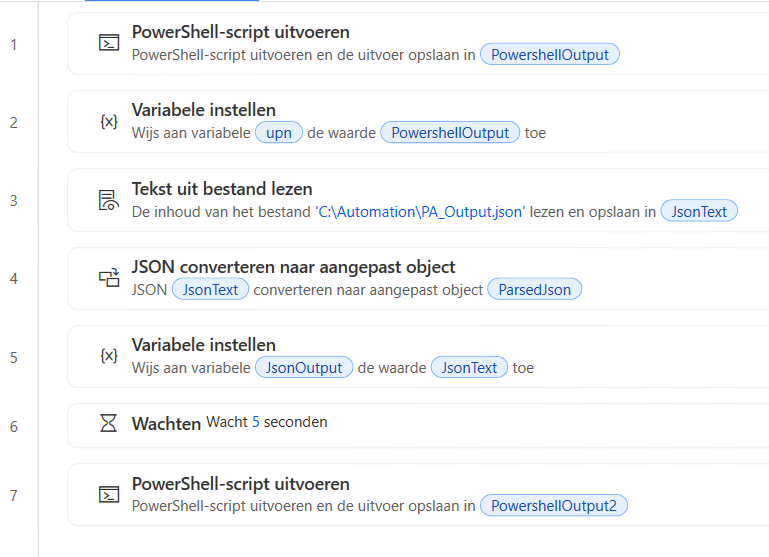
\includegraphics[width=1\textwidth]{DesktopFlow_deel1.png}
    \caption[Desktop flow deel 1]{Eerste flow op de desktop. In deze flow worden de gebruikers aangemaakt en variabelen terug gestuurd naar de cloud flow.}
    \label{fig:DesktopFlow_deel1}
\end{figure}

\section{Cloudverwerking binnen Microsoft 365 en Entra ID}

Deze sectie overloopt de uitwerking van de Entra ID en Microsoft 365 omgeving. 

\subsection{Synchronisatie met Entra ID}

Na het aanmaken van de gebruiker binnen de lokale Active Directory-omgeving moet het account eerst gesynchroniseerd worden naar Microsoft Entra ID voordat bijkomende cloudconfiguraties uitgevoerd kunnen worden. Binnen het gemeentebestuur wordt gebruikgemaakt van een hybride omgeving waarbij lokale Active Directory gekoppeld is aan Microsoft 365 via synchronisatieservices. Er wordt gebruik gemaakt van Entra ID Connect, vroeger ook wel bekend als Azure AD Connect. 

Tijdens deze synchronisatie worden gebruikersaccounts, attributen en groepsgegevens vanuit de lokale Active Directory doorgestuurd naar Entra ID. Hierdoor wordt het lokaal aangemaakte account ook beschikbaar binnen cloudtoepassingen zoals Microsoft 365, Exchange Online en Teams.

Omdat deze synchronisatie niet onmiddellijk gebeurt, kunnen cloudacties zoals het toekennen van licenties of Microsoft 365-groepen niet rechtstreeks uitgevoerd worden na het aanmaken van de gebruiker. De automatiseringsflow moet daarom eerst controleren of het account succesvol beschikbaar geworden is binnen Entra ID.

\subsection{Wachten op synchronisatie}

Om te controleren of de gebruiker succesvol gesynchroniseerd werd naar Entra ID, maakt de cloudflow gebruik van een \texttt{Do Until}-lus binnen Microsoft Power Automate. Deze lus blijft actief totdat het gebruikersaccount beschikbaar wordt binnen de cloudomgeving.

Voordat dit kan gebeuren, moet de aangemaakte UPN van de gebruiker doorgestuurd worden naar de cloudflow. Deze wordt automatisch doorgestuurd door de desktopflow, maar moet eerst nog verwerkt worden in de cloud. Dit gebeurd via de actie ``Parse JSON''. Deze zet de JSON waarde die doorgegeven wordt, via de connectie tussen cloud en desktop, om naar een variabele die normale tekst is. 

Daarna kan de controle starten. Bij het starten van deze controle wordt eerst een booleaanse variabele aangemaakt met de waarde \texttt{false}. Vervolgens probeert de flow via de actie ``Get user profile (V2)'' de gebruiker op te zoeken binnen Entra ID aan de hand van de eerder teruggekoppelde User Principal Name.

Wanneer het gebruikersprofiel succesvol opgehaald kan worden, wordt de variabele aangepast naar \texttt{true}, waardoor de \texttt{Do Until}-lus beëindigd wordt en de volgende cloudconfiguraties uitgevoerd kunnen worden.

Omdat de synchronisatie tussen Active Directory en Entra ID slechts één keer per half uur wordt gestart, werd binnen de lus eveneens een \texttt{Delay}-stap toegevoegd. Hierdoor wordt vermeden dat continu aanvragen naar Entra ID gestuurd worden. Binnen de implementatie wordt telkens 30 seconden gewacht voordat een nieuwe controle uitgevoerd wordt.

\subsection{Toekennen van Microsoft 365-groepen en licenties}

Nadat de gebruiker succesvol gesynchroniseerd werd naar Entra ID, kunnen bijkomende cloudconfiguraties uitgevoerd worden. Binnen de automatiseringsflow worden gebruikers automatisch toegevoegd aan vooraf gedefinieerde Microsoft 365-groepen.

Deze groepen worden gebruikt voor het centraal beheren van toegangsrechten en licenties binnen Microsoft 365. In plaats van licenties rechtstreeks toe te kennen aan individuele gebruikers, zijn de noodzakelijke licenties gekoppeld aan specifieke groepen binnen Entra ID. Wanneer een gebruiker toegevoegd wordt aan een dergelijke groep, worden de gekoppelde licenties automatisch toegewezen.

Binnen de implementatie worden gebruikers standaard toegevoegd aan een algemene Microsoft 365-groep voor E3-licenties die verantwoordelijk is voor de toekenning van basislicenties zoals Exchange Online en Microsoft Teams. Daarnaast wordt eveneens een bijkomende groep toegevoegd voor aanvullende functionaliteiten binnen de organisatie.

De gebruiker wordt naast de groep voor licenties van Microsoft 365 ook nog toegevoegd aan groepen voor een Power Automate licentie en een groep voor toegang tot de VPN. 

Door gebruik te maken van groepsgebaseerde licentietoekenning blijft het beheer eenvoudiger, consistenter en schaalbaarder. Nieuwe gebruikers ontvangen automatisch de correcte cloudconfiguraties zonder dat manuele tussenkomst vereist is.

Figuur ~\ref{fig:Do_until} toont de do until statement die in Power Automate gebruikt wordt.

\begin{figure}[htbp]
    \centering
    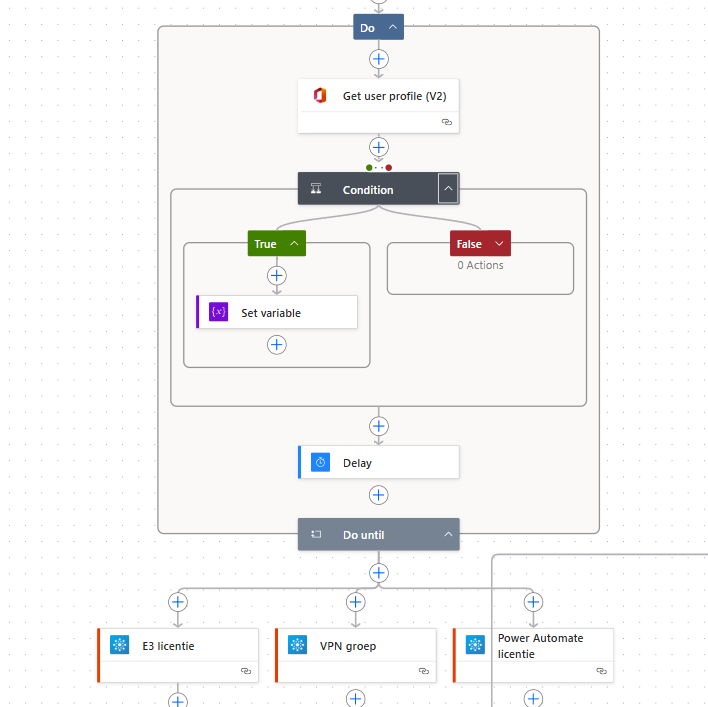
\includegraphics[width=1\textwidth]{Do_Until.png}
    \caption[Controle cloudgebruiker en toevoeging groepen]{Controle of de gebruiker aangemaakt is in Entra ID met de stappen om groepen toe te voegen.}
    \label{fig:Do_until}
\end{figure}

\section{Configuratie van e-mailtoegang}

Na het aanmaken van de gebruiker, de synchronisatie met Entra ID en het toekennen van licenties, worden bijkomende e-mailconfiguraties uitgevoerd. Hierbij gaat het voornamelijk om het toekennen van toegang tot gedeelde postvakken en het toevoegen van gebruikers aan distributiegroepen binnen Microsoft Exchange Online.

De benodigde configuraties worden geselecteerd binnen het Microsoft Forms-formulier tijdens de onboardingaanvraag. Deze gegevens worden vervolgens verwerkt binnen de cloudflow van Power Automate en doorgestuurd naar een bijkomende desktopflow waarin een PowerShell-script uitgevoerd wordt.

Binnen deze automatiseringsstap wordt gebruikgemaakt van de Exchange Online PowerShell-module om rechten toe te kennen op gedeelde postvakken en gebruikers automatisch toe te voegen aan de correcte distributiegroepen.

\subsection{Samenstellen van gedeelde postvakken en distributiegroepen}

Binnen de cloudflow worden de geselecteerde gedeelde postvakken en distributiegroepen opgehaald vanuit het Microsoft Forms-formulier. Omdat gebruikers meerdere opties kunnen selecteren, worden deze waarden verwerkt als lijsten die later doorgestuurd worden naar de desktopflow.

Bij het doorsturen van de informatie zonder ``Compose'' stappen, gaven ze niet altijd de correcte informatie door. Af en toe werden de arrays niet goed opgesteld. Hierdoor werden er toch ``Compose'' stappen toegevoegd zodat de gegevens telkens netjes in correcte arrays terecht kwamen. 

\subsection{Toekennen van mailboxrechten en distributiegroepen}

Omdat Power Automate Cloud geen stappen heeft voor het toekennen van rechten in Exchange Online, wordt er opnieuw gebruik gemaakt van Power Automate Desktop. Er wordt dus een nieuwe desktopflow opgesteld. 

In deze flow, wordt er gebruik gemaakt van de stap ``Toepassing uitvoeren''. De Exchange Online PowerShell module heeft inloggegevens nodig, of een certificaatgebaseerde authenticatie. Wegens tijdsgebrek is de certificaatgebaseerde authenticatie niet geconfigureerd. Dit deel van de oplossing is dus niet volledig geautomatiseerd. Er zullen dus inloggegevens ingevuld worden bij dit deel van de flow.

Het script ontvangt hierbij verschillende parameters vanuit Power Automate, waaronder de User Principal Name van de gebruiker, de geselecteerde gedeelde postvakken en de gekozen distributiegroepen.

Codefragment ~\ref{lst:ExchangeParameters} toont de parameters die vanuit de desktopflow doorgestuurd worden naar het script.

\begin{lstlisting}[language=PowerShell,
    caption={Parameters voor Exchange Online-configuratie},
    label={lst:ExchangeParameters}]
    param(
    [string]$UPN,
    [string]$Mailboxes,
    [string]$DistributionLists
    )
\end{lstlisting}

Voor de communicatie met Exchange Online wordt gebruikgemaakt van de module \texttt{ExchangeOnlineManagement}. Nadat verbinding gemaakt werd met Exchange Online, kan het script rechten en groepslidmaatschappen automatisch configureren.

\begin{lstlisting}[language=PowerShell,
    caption={Verbinding met Exchange Online},
    label={lst:ConnectExchange}]
    Import-Module ExchangeOnlineManagement
    
    Connect-ExchangeOnline -ShowBanner:$false
\end{lstlisting}

De geselecteerde gedeelde postvakken worden eerst verwerkt tot een lijst zodat meerdere mailboxen automatisch verwerkt kunnen worden binnen een lus.

\begin{lstlisting}[language=PowerShell,
    caption={Verwerking van mailboxlijsten},
    label={lst:MailboxList}]
    $MailboxList = $Mailboxes.Trim("[]") -split ","
    
    foreach ($sharedMailbox in $MailboxList) {
        
        $sharedMailbox = $sharedMailbox.Trim(
        " ","'","[","]"
        )
    }
\end{lstlisting}

Voor ieder gedeeld postvak wordt vervolgens automatisch \textit{Full Access}-toegang toegekend aan de gebruiker via het cmdlet \texttt{Add-MailboxPermission}.

\begin{lstlisting}[language=PowerShell,
    caption={Toekennen van mailboxrechten},
    label={lst:MailboxPermissions}]
    Add-MailboxPermission `
    -Identity $sharedMailbox `
    -User $UPN `
    -AccessRights FullAccess `
    -InheritanceType All `
    -Confirm:$false
\end{lstlisting}

Naast volledige toegang wordt eveneens automatisch \textit{Send on Behalf}-toegang ingesteld. Omdat een mailbox hiervoor verplicht is, moet de configuratie van de E3 licentie afgerond zijn. Als deze afgerond is, kunnen de correcte rechten toegewezen worden. Er wordt hierbij gebruikgemaakt van een retry-mechanisme waarbij meerdere pogingen uitgevoerd worden met een tussentijdse wachttijd. Hierdoor worden, op het moment dat de mailbox aangemaakt is, de correcte mailboxen toegewezen aan de gebruiker.

\begin{lstlisting}[language=PowerShell,
    caption={Retry-mechanisme voor Send on Behalf},
    label={lst:RetrySendOnBehalf}]
    while (-not $Success -and $Attempt -lt $MaxAttempts) {
        
        try {
            
            Set-Mailbox `
            -Identity $sharedMailbox `
            -GrantSendOnBehalfTo @{Add=$UPN}
            
            $Success = $true
        }
        catch {
            
            $Attempt++
            
            Start-Sleep -Seconds 60
        }
    }
\end{lstlisting}

\subsection{Toevoegen aan distributiegroepen}

Naast gedeelde postvakken worden gebruikers eveneens automatisch toegevoegd aan distributiegroepen binnen Exchange Online. Hierbij worden zowel standaard distributiegroepen als bijkomende groepen uit het formulier verwerkt.

\begin{lstlisting}[language=PowerShell,
    caption={Standaard distributiegroepen},
    label={lst:DefaultDLs}]
    $DefaultDLs = @(
    "iedereen@berlare.be",
    "viruswaarschuwing@berlare.be"
    )
\end{lstlisting}

Tot slot worden alle distributiegroepen doorlopen en wordt de gebruiker automatisch toegevoegd via het cmdlet \texttt{Add-DistributionGroupMember}.

\begin{lstlisting}[language=PowerShell,
    caption={Toevoegen aan distributiegroepen},
    label={lst:AddDistributionGroup}]
    Add-DistributionGroupMember `
    -Identity $dl `
    -Member $UPN `
    -BypassSecurityGroupManagerCheck
\end{lstlisting}

Door deze configuraties automatisch uit te voeren, wordt het manuele beheer van mailboxrechten en distributiegroepen sterk verminderd en verloopt de onboarding consistenter en efficiënter.

\section{Foutafhandeling en betrouwbaarheid}

Binnen de verschillende PowerShell-scripts wordt gebruikgemaakt van foutafhandeling om onverwachte problemen gecontroleerd op te vangen zonder dat het volledige onboardingproces abrupt stopt. Hiervoor worden voornamelijk \texttt{try-catch}-constructies gebruikt.

Wanneer een fout optreedt tijdens het uitvoeren van een opdracht, wordt een waarschuwing of foutmelding weggeschreven zodat deze later geraadpleegd kan worden binnen Power Automate of tijdens troubleshooting. Dit zorgt er echter niet voor dat de flow automatisch stopt.

Codefragment ~\ref{lst:MailboxErrorHandling} toont een voorbeeld van foutafhandeling tijdens het toevoegen van een gebruiker aan een gedeeld postvak.

\begin{lstlisting}[language=PowerShell,
    caption={Foutafhandeling bij mailboxrechten},
    label={lst:MailboxErrorHandling}]
    try {
        
        Add-MailboxPermission `
        -Identity $sharedMailbox `
        -User $UPN `
        -AccessRights FullAccess `
        -ErrorAction Stop
    }
    catch {
        
        Write-Warning "Failed FullAccess"
        Write-Warning $_.Exception.Message
    }
\end{lstlisting}

Daarnaast wordt binnen bepaalde onderdelen gebruikgemaakt van retry-mechanismen. Dit is voornamelijk noodzakelijk bij synchronisatieprocessen binnen Exchange Online en Entra ID, waarbij objecten niet altijd onmiddellijk beschikbaar zijn na het aanmaken van een gebruiker.

Door meerdere pogingen uit te voeren met een tussentijdse wachttijd, kan het script tijdelijke synchronisatieproblemen automatisch opvangen zonder manuele tussenkomst.

\begin{lstlisting}[language=PowerShell,
    caption={Retry-mechanisme},
    label={lst:RetryMechanism}]
    while (-not $Success -and $Attempt -lt $MaxAttempts) {
        
        try {
            
            Set-Mailbox `
            -Identity $sharedMailbox `
            -GrantSendOnBehalfTo @{Add=$UPN}
            
            $Success = $true
        }
        catch {
            
            $Attempt++
            
            Start-Sleep -Seconds 60
        }
    }
\end{lstlisting}

Deze aanpak verhoogt de betrouwbaarheid van het onboardingproces en vermindert de nood aan manuele correcties wanneer tijdelijke fouten of synchronisatievertragingen optreden.

\section{Automatische terugkoppeling via e-mail}

Na het succesvol uitvoeren van de onboardingflow wordt automatisch een e-mail verstuurd vanuit een gedeeld postvak van de ICT-dienst. Deze e-mail bevat bijkomende informatie en handleidingen voor de nieuwe medewerker.

In deze handleidingen zijn stappenplannen te vinden met betrekking tot het gebruik van de VPN, het vrijgeven van e-mails die tegengehouden worden door de spamfilter en printen. In de e-mail zelf zijn ook een paar praktische afspraken in verband met het gebruik van wifi. Ook de uitleg over MFA is te vinden in deze e-mail. Ook is er in de e-mail een link naar de helpdesk waar ze al hun problemen moeten melden en uiteraard ook geholpen worden indien nodig. 

Binnen Power Automate moeten deze bijlagen eerst geladen worden. Dit gebeurd met de stap ``Get file content''. Voor de 4 bijlagen gebeurt dit dus op identieke, parallelle wijze. Eens deze opgeladen zijn in Power Automate, kunnen ze geselecteerd worden in de stap ``Send an email from a shared mailbox''. Hierin staat het e-mailadres dat de e-mail verstuurt, als ook de ontvanger. Dit is op dynamische wijze opnieuw de UPN variabele die initieel via de desktopflow naar de cloud wordt gestuurd. Net zoals bij een normale e-mail hoort er ook een onderwerp en de gehele e-mail bij. 

Figuur ~\ref{fig:Mails} toont hoe de bijlagen worden aangemaakt en hoe de e-mail verstuurd wordt.

\begin{figure}[htbp]
    \centering
    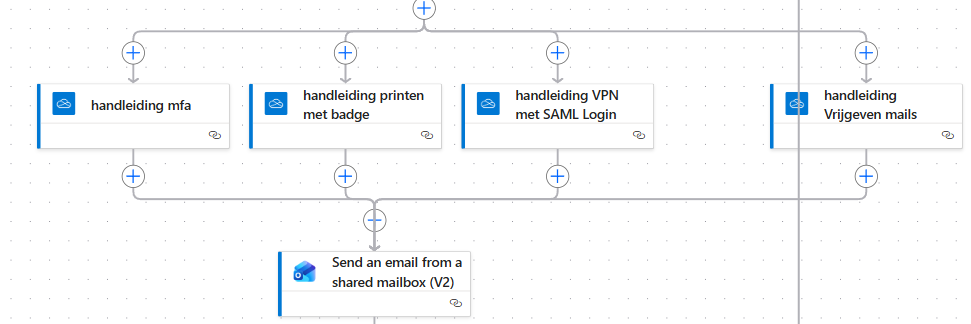
\includegraphics[width=1\textwidth]{Mails.png}
    \caption[Stappen om een e-mail te versturen]{Stappen die nodig zijn in een flow om een automatische e-mail met bijlagen te versturen}
    \label{fig:Mails}
\end{figure}

\section{Logging van uitgevoerde onboardings}

Om opvolging en controle mogelijk te maken, wordt na een succesvolle onboarding automatisch een logregistratie toegevoegd binnen een Excelbestand. Deze registratie bevat onder andere de naam van de gebruiker, de uitvoeringsdatum en de status van de onboarding.

Binnen de cloudflow wordt hiervoor gebruikgemaakt van de actie ``Update a row''. Hiermee wordt de bestaande aanvraag bijgewerkt zodat zichtbaar wordt dat de onboarding succesvol uitgevoerd werd.

Door gebruik te maken van deze logging kan de ICT-dienst eenvoudig controleren welke onboardings reeds uitgevoerd werden en kunnen eventuele problemen later sneller opgespoord worden. Ook voor de medewerkers van andere diensten is dit handig om te zien of alles van IT in orde is voor de nieuwe collega.

Figuur ~\ref{fig:Voorbeeld_output_logging} toont het loggen wanneer de gebruiker aangemaakt is.

\begin{figure}[htbp]
    \centering
    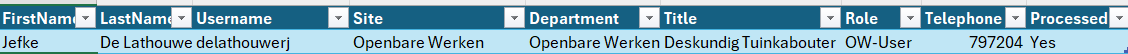
\includegraphics[width=1\textwidth]{VoorbeeldoutputLogging.png}
    \caption[Voorbeeld output van logging]{Aangepaste rij nadat de gebruiker is aangemaakt. Kolom ``Processed'' is veranderd van ``No'' naar ``Yes''}
    \label{fig:Voorbeeld_output_logging}
\end{figure}

\section{Geautomatiseerde offboarding van gebruikers}

Naast het onboardingproces werd eveneens een geautomatiseerde offboardingflow ontwikkeld binnen Microsoft Power Automate. Deze flow zorgt ervoor dat gebruikersaccounts en bijhorende configuraties automatisch aangepast worden wanneer een medewerker de organisatie verlaat.

De offboarding start vanuit een afzonderlijk Microsoft Forms-formulier waarin onder andere de User Principal Name van de gebruiker, de einddatum van het contract en de reden van uitdiensttreding ingevuld worden. Nadat het formulier verzonden werd, start automatisch een cloudflow binnen Power Automate die de verdere verwerking uitvoert.

Net zoals bij de onboarding wordt gebruikgemaakt van een hybride aanpak waarbij cloudflows gecombineerd worden met desktopflows en PowerShell-scripts. Hierdoor kunnen zowel cloudconfiguraties binnen Microsoft 365 als lokale configuraties binnen Active Directory automatisch aangepast worden.

Tijdens de offboarding worden verschillende acties uitgevoerd. Hierbij wordt de mailbox van de gebruiker eerst omgezet naar een gedeeld postvak waarna rechten op gedeelde postvakken en distributiegroepen verwijderd worden. Vervolgens wordt het Active Directory-account gedeactiveerd, verborgen uit de globale adreslijst en verwijderd uit beveiligingsgroepen en andere groepslidmaatschappen.

Daarnaast worden ook Microsoft 365-groepen aangepast zodat gekoppelde licenties automatisch vrijgegeven worden. Door deze stappen automatisch uit te voeren, verloopt de offboarding consistenter en wordt de nood aan manuele tussenkomst verminderd.

\subsection{Cloudflow voor offboarding}

De offboardingflow start binnen Microsoft Power Automate wanneer een nieuwe reactie verzonden wordt via het Microsoft Forms-formulier voor offboarding. Net zoals bij de onboarding worden de ingevulde gegevens automatisch opgehaald aan de hand van het unieke reactie-id van het formulier.

Na het ophalen van de gegevens wordt gecontroleerd welke einddatum voor de medewerker werd opgegeven. Deze datum bepaalt wanneer de effectieve offboarding uitgevoerd mag worden. Zolang de einddatum nog niet bereikt werd, blijft de flow in wachtstatus staan zodat de verdere automatiseringsstappen nog niet uitgevoerd worden.

Deze aanpak voorkomt dat een gebruikersaccount te vroeg gedeactiveerd wordt terwijl de medewerker nog actief is binnen de organisatie. Aangezien de personeelsdienst de einddatum reeds kent bij het registreren van de uitdiensttreding, kan deze informatie vooraf meegegeven worden binnen het formulier.

Binnen de cloudflow wordt hiervoor gebruikgemaakt van een wachttijd op basis van datum en tijd. Zodra de opgegeven einddatum bereikt wordt, hervat de flow automatisch en worden de verdere offboardingstappen uitgevoerd.

\subsection{Desktopflow en verwerking binnen Exchange Online}

Wanneer de opgegeven einddatum bereikt werd, start de cloudflow automatisch een desktopflow binnen Power Automate Desktop. Deze desktopflow is verantwoordelijk voor het uitvoeren van de PowerShell-scripts die de effectieve offboarding van de gebruiker uitvoeren binnen Exchange Online.

Net zoals bij de onboarding wordt gebruikgemaakt van een hybride aanpak waarbij Power Automate Cloud communiceert met de lokale infrastructuur via Power Automate Desktop en Power Automate Machine Runtime. Hierdoor kunnen lokale Active Directory-configuraties gecombineerd worden met cloudconfiguraties binnen Microsoft 365.

Vanuit de cloudflow worden verschillende parameters doorgestuurd naar de desktopflow, waaronder de User Principal Name van de gebruiker, de reden van uitdiensttreding en de einddatum van het contract.

Codefragment ~\ref{lst:OffboardingExchangeParameters} toont de parameters die gebruikt worden binnen het Exchange Online-script.

\begin{lstlisting}[language=PowerShell,
    caption={Parameters voor Exchange Online-offboarding},
    label={lst:OffboardingExchangeParameters}]
    param(
    [string]$UPN
    )
\end{lstlisting}

Binnen het script wordt eerst verbinding gemaakt met Exchange Online via de module \texttt{ExchangeOnlineManagement}. Hierdoor kunnen mailboxen, rechten en distributiegroepen automatisch aangepast worden tijdens de offboarding.

\begin{lstlisting}[language=PowerShell,
    caption={Verbinding met Exchange Online},
    label={lst:ConnectExchangeOffboarding}]
    Import-Module ExchangeOnlineManagement
    
    Connect-ExchangeOnline
\end{lstlisting}

\subsubsection{Omzetten naar gedeeld postvak}

De mailbox van de gebruiker wordt eerst automatisch omgezet naar een gedeeld postvak. Hierdoor blijven bestaande e-mails en agenda-items behouden nadat de gebruiker uit dienst gegaan is.

\begin{lstlisting}[language=PowerShell,
    caption={Omzetten naar gedeeld postvak},
    label={lst:ConvertSharedMailbox}]
    Set-Mailbox `
    -Identity $UserMailbox.PrimarySmtpAddress `
    -Type Shared
\end{lstlisting}

Door de mailbox om te zetten naar een gedeeld postvak kan de Microsoft 365-licentie later verwijderd worden zonder dat historische communicatie verloren gaat. Dit maakt het mogelijk om oude e-mails nog tijdelijk te raadplegen indien nodig.

\subsubsection{Verwijderen van mailboxrechten en distributiegroepen}

Na het omzetten van de mailbox worden bestaande rechten en groepslidmaatschappen verwijderd. Hierbij wordt eerst gecontroleerd op mailboxen waarvoor de gebruiker \textit{Full Access}-rechten bezit.

\begin{lstlisting}[language=PowerShell,
    caption={Verwijderen van Full Access-rechten},
    label={lst:RemoveFullAccess}]
    Remove-MailboxPermission `
    -Identity $Mailbox.PrimarySmtpAddress `
    -User $UPN `
    -AccessRights FullAccess `
    -Confirm:$false
\end{lstlisting}

Daarnaast wordt eveneens gecontroleerd of de gebruiker \textit{Send on Behalf}-rechten bezit op andere mailboxen. Indien deze rechten aanwezig zijn, worden ze automatisch verwijderd.

\begin{lstlisting}[language=PowerShell,
    caption={Verwijderen van Send on Behalf},
    label={lst:RemoveSendOnBehalf}]
    Set-Mailbox `
    -Identity $Mailbox.PrimarySmtpAddress `
    -GrantSendOnBehalfTo @{
        Remove = $UserMailbox.DistinguishedName
    }
\end{lstlisting}

Tot slot wordt de gebruiker automatisch verwijderd uit distributiegroepen binnen Exchange Online.

\begin{lstlisting}[language=PowerShell,
    caption={Verwijderen uit distributiegroepen},
    label={lst:RemoveDistributionGroups}]
    Remove-DistributionGroupMember `
    -Identity $_.PrimarySmtpAddress `
    -Member $UPN `
    -Confirm:$false
\end{lstlisting}

Door deze rechten en groepslidmaatschappen automatisch te verwijderen, wordt vermeden dat voormalige medewerkers nog toegang behouden tot gedeelde mailboxen of interne communicatiestromen.

\subsection{Desktopflow en verwerking binnen Active Directory}

Naast de configuraties binnen Exchange Online worden tijdens de offboarding eveneens verschillende aanpassingen uitgevoerd binnen de lokale Active Directory-omgeving. Hiervoor wordt een tweede PowerShell-script uitgevoerd vanuit Power Automate Desktop.

Dit script ontvangt verschillende parameters vanuit de cloudflow, waaronder de User Principal Name van de gebruiker, de reden van uitdiensttreding en de einddatum van het contract.

Codefragment ~\ref{lst:ADOffboardingParameters} toont de parameters die gebruikt worden binnen het Active Directory-script.

\begin{lstlisting}[language=PowerShell,
    caption={Parameters voor Active Directory-offboarding},
    label={lst:ADOffboardingParameters}]
    param(
    [string]$UPN,
    [string]$Reason,
    [string]$EndDate
    )
\end{lstlisting}

Binnen het script wordt eerst gecontroleerd of het gebruikersaccount effectief bestaat binnen Active Directory. Hiervoor wordt de gebruiker opgezocht aan de hand van de User Principal Name.

\begin{lstlisting}[language=PowerShell,
    caption={Opzoeken van de gebruiker},
    label={lst:GetADUserOffboarding}]
    $User = Get-ADUser `
    -Filter "UserPrincipalName -eq '$UPN'" `
    -Properties MemberOf,Description
\end{lstlisting}

Na het ophalen van het account kunnen de verdere offboardingstappen automatisch uitgevoerd worden.

\subsubsection{Deactiveren van gebruikersaccounts}

Tijdens de offboarding wordt het gebruikersaccount automatisch gedeactiveerd binnen Active Directory. Hierdoor kan de voormalige medewerker niet langer aanmelden binnen de omgeving van de organisatie.

\begin{lstlisting}[language=PowerShell,
    caption={Deactiveren van gebruikersaccounts},
    label={lst:DisableADAccount}]
    Disable-ADAccount -Identity $User
\end{lstlisting}

Daarnaast wordt het account verborgen uit de Global Address List van Exchange. Hierdoor verschijnt de gebruiker niet langer binnen adreslijsten van Microsoft Outlook of andere Microsoft 365-toepassingen.

\begin{lstlisting}[language=PowerShell,
    caption={Verbergen uit de Global Address List},
    label={lst:HideFromGAL}]
    Set-ADUser `
    -Identity $User `
    -Replace @{
        msExchHideFromAddressLists=$true
    }
\end{lstlisting}

Naast het uitschakelen van het account wordt eveneens de beschrijving van de gebruiker aangepast. Hierbij wordt automatisch geregistreerd vanaf wanneer de medewerker uit dienst is en wat de reden van uitdiensttreding was.

\begin{lstlisting}[language=PowerShell,
    caption={Aanpassen van de beschrijving},
    label={lst:DescriptionOffboarding}]
    $NewDescription = 
    "Uit dienst sinds $FormattedDate - $Reason"
    
    Set-ADUser `
    -Identity $User `
    -Description $NewDescription
\end{lstlisting}

Door deze informatie rechtstreeks binnen Active Directory op te slaan, blijft bijkomende administratieve informatie beschikbaar voor de ICT-dienst en systeembeheerders.

\subsubsection{Verwijderen van groepslidmaatschappen}

Na het deactiveren van het account worden bestaande groepslidmaatschappen automatisch verwijderd. Hierdoor verliest de gebruiker alle gekoppelde rechten en toegangen binnen de infrastructuur van de organisatie.

Binnen het script wordt eerst een beperkte lijst samengesteld van groepen die behouden moeten blijven. In de huidige implementatie blijft enkel de standaardgroep \texttt{Domain Users} behouden.

\begin{lstlisting}[language=PowerShell,
    caption={Groepen die behouden blijven},
    label={lst:GroupsToKeep}]
    $GroupsToKeep = @(
    "Domain Users"
    )
\end{lstlisting}

Vervolgens worden alle groepslidmaatschappen van de gebruiker opgehaald en gecontroleerd. Indien een groep niet voorkomt binnen de uitzonderingslijst, wordt de gebruiker automatisch uit deze groep verwijderd.

\begin{lstlisting}[language=PowerShell,
    caption={Verwijderen van groepslidmaatschappen},
    label={lst:RemoveADGroups}]
    Remove-ADGroupMember `
    -Identity $_ `
    -Members $User `
    -Confirm:$false
\end{lstlisting}

Door groepslidmaatschappen automatisch te verwijderen, wordt vermeden dat voormalige medewerkers nog toegang behouden tot netwerkshares, beveiligingsgroepen of andere interne systemen die gekoppeld zijn aan Active Directory-groepen.

Net zoals bij de onboarding wordt ook binnen deze scripts gebruikgemaakt van \texttt{try-catch}-constructies zodat fouten gecontroleerd opgevangen kunnen worden zonder dat het volledige proces abrupt stopt.

Figuur ~\ref{fig:DesktopOffboarding} toont de complete desktopflow voor het offboardingsproces.

\begin{figure}[htbp]
    \centering
    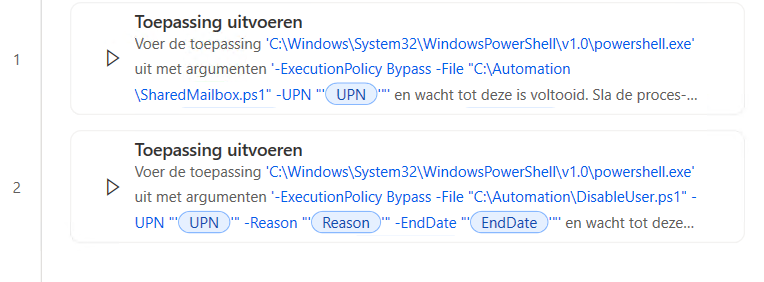
\includegraphics[width=1\textwidth]{DesktopOffboarding.png}
    \caption[Desktopflow offboarding]{Desktopflow voor het offboardingsproces}
    \label{fig:DesktopOffboarding}
\end{figure}

\subsection{Verwijderen van groepslidmaatschappen en licenties}

Naast de lokale Active Directory-groepen moeten tijdens de offboarding eveneens verschillende cloudgroepen binnen Microsoft 365 verwijderd worden. Deze groepen werden tijdens de onboarding automatisch toegekend via Power Automate en zijn verantwoordelijk voor het toewijzen van licenties en bijkomende toegangsrechten.

Binnen de implementatie gaat het onder andere om de Microsoft 365 E3-licentie, een Power Automate-licentie en een groep die toegang verleent tot de VPN-omgeving van de organisatie.

Het verwijderen van deze groepen gebeurt volledig binnen de cloudflow van Power Automate. Hiervoor wordt gebruikgemaakt van de actie ``Lid uit groep verwijderen''. Via deze stap wordt de gebruiker automatisch verwijderd uit de vooraf gedefinieerde Microsoft 365-groepen.

Voor het identificeren van de gebruiker wordt het e-mailadres gebruikt dat eerder via het formulier en de desktopflow verwerkt werd. Hierdoor kan de correcte gebruiker automatisch opgezocht en verwijderd worden uit de overeenkomstige groepen binnen Entra ID.

Door gebruikers automatisch uit deze groepen te verwijderen, worden gekoppelde licenties en toegangsrechten eveneens automatisch ingetrokken. Dit vermindert het risico op ongewenste toegang na uitdiensttreding en zorgt ervoor dat ongebruikte licenties opnieuw beschikbaar worden binnen de organisatie. Dit is dus zowel positief voor veiligheid van gegevens, als ook voor het niet verspillen van licenties. \newline

Figuur ~\ref{fig:CloudOffboarding} toont de complete cloudflow voor het offboardingsproces.

\begin{figure}[htbp]
    \centering
    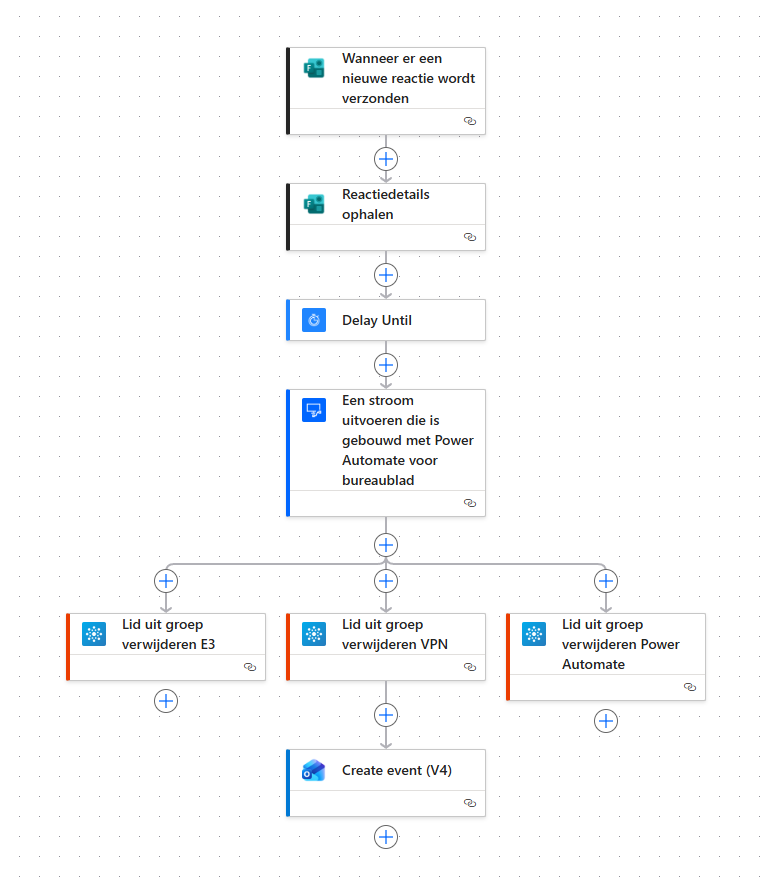
\includegraphics[width=0.8\textwidth]{CloudOffboarding.png}
    \caption[Cloudflow offboarding]{Cloudflow voor het offboardingsproces}
    \label{fig:CloudOffboarding}
\end{figure}

%Om een automatische werking op te stellen, werd door een collega gekozen voor Power Automate. Power Automate is een programma van Microsoft zelf dat gebruikt kan worden om automatische flows te maken. Power automate is voornamelijk een tool dat in de cloud draait, maar het kan ook voor automatisatie zorgen on prem. \newline

%Voor cloud toepassingen van Microsoft heeft Power Automate verschillende stappen. Zo kan je echt op vlak van gebruikers mensen gaan aanmaken in Entra ID en deze aan groepen toevoegen etc. Aangezien er in de gemeente gebruik wordt gemaakt van een hybride omgeving, met dus zowel toepassing van Active Directory in de cloud en on prem, is het dus belangrijk dat de gebruikers on prem worden aangemaakt. \newline

%Voor active directory heeft Power Automate geen speciale stappen die je kan gebruiken. Hiervoor wordt het script, dat in hoofdstuk ~\ref{ch:analyseontwerp} uitgelegd wordt, gebruikt. Dit script staat dus lokaal op een server opgeslagen. Aangezien Power Automate een cloud tool is, is er de desktop versie van Power Automate nodig. Deze applicatie werkt als brug tussen de online versie en de lokale toepassing van de Active Directory. \newline

%In de cloud is er een flow gemaakt. Deze flow start met het ophalen van gegevens wanneer er een nieuwe inzending is van het formulier. Hiervoor is een stap die voorzien is, namelijk de stap ``Wanneer er een nieuwe reactie wordt verzonden''. In deze stap kan je eenvoudig in een keuze menu kiezen voor het formulier dat je in Microsoft Forms hebt gemaakt. Als deze er niet bijstaat, kan je ook op zoek gaan naar het id van het formulier. Deze kan je vinden in de URL van jouw form, achter het duidelijke ``FormID'' in de URL. \newline

%Hierna moet er nog een stap komen met de gemaakte form. Hiervoor heb je de stap ``Reactiedetails ophalen''. Hierin moet je opnieuw het id van de form ingeven, als ook het id van het antwoord kiezen. Bij het antwoord moet je kiezen voor een dynamische expressie te kiezen. Op deze manier kan je de laatst verzonden input selecteren. Je kan de dynamische expressie kiezen door aan de rechterkant van de kolom op de bliksemschicht te klikken, of door een ``/'' te typen.\newline

%De gemeente heeft, zoals uitgelegd in hoofdstuk ~\ref{ch:analyseontwerp}, op verschillende niveaus gebruikers. Ze zitten allemaal in een ``OU'' ``Users'', maar ze zitten wel nog steeds, afhankelijk van de sites, 1 niveau verschil. Hiervoor in binnen Power Automate, een extra stap gemaakt om de juiste sites en diensten toe te kennen. Hiervoor is de stap ``Compose'' aangeroepen. 

%Deze ``Compose'' gaat bij de vraag van welke site, kijken naar de reactie. Op vlak daarvan gaat hij het antwoord van de vraag over welke dienst de gebruiker zit. Zo gaat de form bijvoorbeeld bij het selecteren van site ``Gemeentehuis'', naar de vraag voor welke diensten van site gemeentehuis. Hierin staan dan bijvoorbeeld diensten ``vergunningen, personeelsdienst of informatica''. In de IF-statement kijkt hij bij het selecteren dan naar die vraag. Dit zorgt er voor dat hij dus altijd voor de dienst, de correcte dienst die in de form wordt gekozen, wordt ingevuld. Om het heel simpel uit te leggen, de IF-statements simuleren de werking van het formulier dat over bepaalde stappen springt afhankelijk van de antwoorden die worden gekozen. \newline

%Omdat Power Automate een betalende licentie heeft, werd er eerst een tussenstap gemaakt. De gegevens werden naar een Excel gestuurd. In deze Excel werden de kolommen exact hetzelfde aangemaakt als in de test Excel voor het script. Deze zorgden voor een duidelijke verwerking van de gegevens. Op deze manier kon er ook eenvoudig gecontroleerd worden of de gebruikers de correcte gegevens meekregen. Dit was een tijdelijke, noodzakelijke tussenstap. \newline



%De volgende stap is het script op de server aanroepen. Dit kan je doen door een stap toe te voegen in de cloud. De stap heeft de naam ``Run a flow built with Power Automate for desktop''. Hierin kan je een flow kiezen, die je op de desktop gemaakt hebt. 

%Om dit te kunnen doen moet je uiteraard een desktop hebben om deze flow op te runnen. Hiervoor moet ``Power automate desktop'' geïnstalleerd worden. Dit kan gewoon via de website van Microsoft. Eens geïnstalleerd, moet je inloggen met het account waarmee je ook in de cloud bent ingelogd. Hierna kan je een flow maken. Je kan de flow uiteindelijk ook zien staan in de cloud, maar zal deze nooit kunnen bewerken in de cloud. Dit moet on-premesis gebeuren.

%Om een connectie te maken tussen de cloud versie van Power Automate en de desktop versie, moet je een andere applicatie gebruiken.  Hiervoor wordt de applicatie ``Power automate machine runtime'' gebruikt. Deze geeft meteen de correcte omgeving weer, waarin je aan het werken bent. Ook al geeft deze de correcte omgeving weer, wilt dit niet zeggen dat er al een connectie is. Hiervoor moet je op de knop ``Refresh'' drukken. Hierdoor maakt de machine dan connectie met het internet en met jouw cloud. 

%Eens dit is gedaan, kan je aan de flow beginnen. De flow in de desktop versie is redelijk simpel. Deze roept het script, dat lokaal opgeslagen staat op dezelfde computer of server, aan. Hiervoor wordt de stap ``Run PowerShell Script'' gebruikt. In deze stap wordt het script aangeroepen vanop de locatie waar het staat. Bij het script horen ook variabelen. Deze dienen ook aangemaakt te worden in de desktop applicatie. Deze variabelen hebben exact dezelfde naam als de gegevens die worden toegewezen in de cloud versie. Op deze manier kunnen ze aan elkaar gelinkt worden.

%De volgende stappen in de desktop versie, zijn enkel om de correcte gebruikersnaam door te geven aan de cloud. Dit is nodig omdat de gebruiker in de cloud ook toegevoegd wordt aan groepen. Hiervoor is de correcte naam nodig, deze wordt dan ook vanuit de desktop versie doorgegeven aan de cloud versie om de foutmarge zo klein mogelijk te maken.

%Verder is er nog 1 stap die in de desktop versie moet gebeuren. Deze stap zorgt ervoor dat de gebruiker bij tijdelijke contracten ook een einddatum krijgen in de Active Directory. Om veiligheidsredenen wordt dit nu handmatig gedaan als er een gekende einddatum is, maar bij een automatisch proces, gebeurt dat het beste automatisch. Deze stap zit niet in het script verwerkt aangezien de code om dit te doen, niet werkt in het script maar wel daar buitenom. Een verklaring hiervoor is niet gevonden. \newline

%Hierna moet dan nog de laatste stappen gebeuren voor de nieuwe gebruiker. Het toekennen van licentiesin entra id. Dit gebeurt door de licenties toe te kennen aan groepen en gebruikers dan in deze groepen te plaatsen. Voordat dit kan gebeuren, moet de gebruiker aangemaakt worden in de cloud. Dit kan eenvoudig gebeuren door eerst een variabele aan te maken. Dit hoort een boolean te zijn. Deze waarde moet op false staan. 

%Hierna komt de grootste stap. Om de loop te maken moet de stap ``Do Until'' aangeroepen worden. Deze stap werkt eigenlijk zoals een do while in andere programmeertalen. Deze stap gaat controleren of de variabele van waarde is veranderd. Van false naar true dus. Binnen deze stap, zitten verschillende andere stappen. Zo wordt er eerst gekeken of de gebruiker aangemaakt is in ``Entra ID'', de opvolger van ``Azure AD''. De stap ``Get user profile (V2)'' wordt hiervoor gebruikt. Deze haalt gegevens op uit Entra ID. In de flow wordt dan de mail van de nieuwe gebruiker meegegeven. Als deze bestaat, zullen de gegevens in de output van dit object komen.Hierna wordt er een condition aangeroepen als stap. Deze stap gaat kijken of er een object van het user profiel uit de vorige stap, bestaat. Als deze niet leeg is, dan wilt het dus zeggen dat hij aangemaakt is. Hierna wordt de variabele aangepast van false naar true en zal de ``Do Until'' eindigen en zullen de volgende stappen uitgevoerd worden. 

%Stel dat de user nog niet zou bestaan, gaat de ``Get user profile'' stap een foutmelding geven. Deze error kan je omzeilen door te zeggen dat de condition moet blijven lopen, ook als de stap ervoor een foutmelding geeft. 

%Verder moet er nog een ``Delay'' stap komen. Deze stap zorgt dat de flow niet iedere seconde een vraag stuurt of deze al bestaat. Mocht dit wel zo zijn, zou er een te grote hoeveelheid aan vragen zijn en zou de flow blokkeren. De vertraging staat ingesteld op iedere 30 seconden en zal 120 keer lopen. Dit om zeker te zijn dat de automatische synchronisatie cyclus zeker voldoende tijd heeft om te lopen. Deze loopt 1 keer per half uur. \newline

%De laatste stappen zijn dan om de gebruiker toe te voegen aan de correcte groepen in Entra. Dit zijn groepen die licenties meegeven. Dit gebeurt met de stap ``Office 365 Groups''. Deze worden toegevoegd op vlak van het group-id in Entra en de User Principal Name. \newline

%Eventueel kan er daarna nog een stap komen om terug te koppelen naar het algemene systeem voor de onboarding. Momenteel kan dit nog niet toegepast worden, aangezien hiervoor nog geen systeem bestaat en dit ook nog in productie zit. \newline

%Figuur \ref{fig:PowerAutomateCloud} toont een visuele voorstelling van de PowerAutomate flow.

%\begin{figure}[htbp]
%\centering
%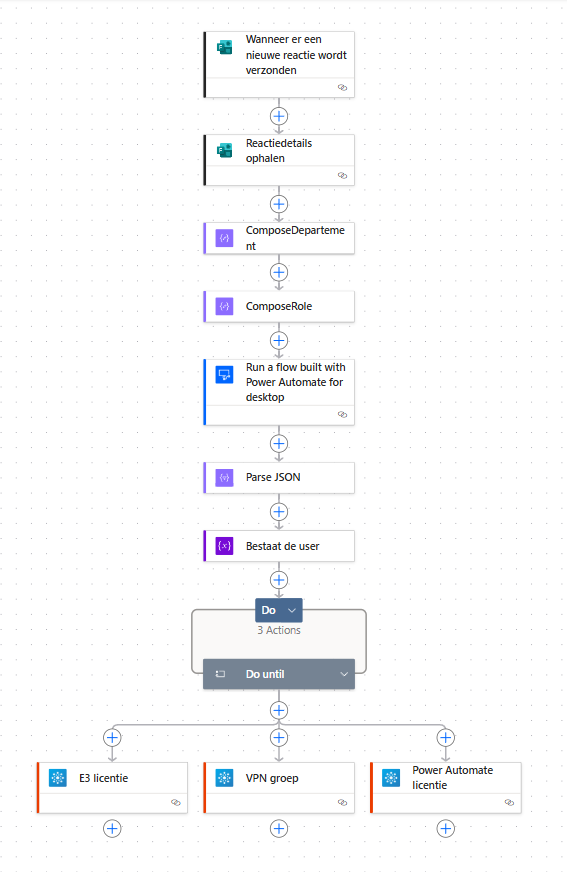
\includegraphics[width=0.8\textwidth]{PowerAutomate.png}
%\caption[Complete Power Automate Cloud flow]{Deze afbeelding is de complete flow die in de cloud is. Deze flow heeft alle tussenstappen die hierboven beschreven zijn en waar er duidelijk vermeld staat dat het een cloud stap is. }
%\label{fig:PowerAutomateCloud}
%\end{figure}

%%
%%Implementatie van de oplossing
%%

\chapter{Evaluatie}
\label{ch:Evaluatie}

In dit hoofdstuk worden de automatiseringsprocessen geëvalueerd.

\section{Evaluatie van de onboardingautomatisering}

In deze sectie wordt het onboardingsproces geëvalueerd.

\subsection{Vergelijking van het manuele en geautomatiseerde proces}

Het oorspronkelijke onboardingproces van het lokaal gemeentebestuur van Berlare verliepen alle stappen volledig manueel. Zowel het aanmaken van gebruikersaccounts als het toekennen van rechten, groepslidmaatschappen en licenties moesten handmatig uitgevoerd worden door medewerkers van de ICT-dienst.

Deze werkwijze was tijdrovend en zorgde ervoor dat medewerkers van de ICT-dienst een aanzienlijk deel van hun tijd moesten besteden aan repetitieve administratieve taken. Hierdoor bleef minder tijd beschikbaar voor complexere technische problemen en andere ondersteunende opdrachten binnen de organisatie. Ook werd de onboarding vaak vooraf niet doorgegeven. Daardoor moest er meteen geschakeld worden om het in orde te brengen en moesten de andere taken aan de kant geschoven worden. 

Door automatisatie via Microsoft Power Automate en PowerShell wordt een groot deel van deze manuele tussenkomsten geëlimineerd. De personeelsdienst kan nu zelfstandig een onboardingaanvraag starten via Microsoft Forms, waarna de verdere verwerking grotendeels automatisch verloopt.

Initieel werden gebruikersaccounts eerst handmatig aangemaakt binnen Active Directory. Vervolgens moesten gebruikers afzonderlijk toegevoegd worden aan de correcte groepen en Organizational Units. Nadien moest gewacht worden tot de synchronisatie met Microsoft 365 afgerond was voordat bijkomende cloudconfiguraties uitgevoerd konden worden. Ook het toekennen van licenties gebeurde manueel. Ook de rechten op mailboxen en distributiegroepen gebeurde handmatig.

Binnen de geautomatiseerde oplossing worden deze configuraties automatisch uitgevoerd op basis van de gegevens die ingevuld worden binnen het onboardingformulier. Hierdoor verloopt het volledige proces sneller, consistenter en met een kleinere kans op menselijke fouten.

Als laatste werd ook de communicatie handmatig gedaan. Interne communicatie is een werkpunt voor de gemeente en daardoor wordt het soms vergeten. Aangezien de communicatie handmatig gebeurde, alsook soms vergeten werd, waren vaak andere collega's niet op de hoogte van de status. Met de automatische terugkoppeling die in dit project werd geconfigureerd, wordt de communicatie consistenter en betrouwbaarder. 

In tabel~\ref{tab:VergelijkingOnboarding} vind je een overzichtelijke vergelijking tussen het manuele en geautomatiseerde proces.

\begin{table}[htbp]
    \centering    
    \begin{tabular}{|p{4cm}|p{5cm}|p{5cm}|}
        \hline
        \textbf{Processtap} & \textbf{Manueel proces} & \textbf{Geautomatiseerd proces} \\
        \hline
        
        Gebruiker aanmaken &
        Handmatig via Active Directory Users and Computers &
        Automatisch via PowerShell-script \\
        \hline
        
        Groepslidmaat-schappen &
        Handmatig toevoegen per gebruiker &
        Automatisch via rolgebaseerde mappings \\
        \hline
        
        Licenties toekennen &
        Handmatig toevoegen aan cloudgroepen &
        Automatisch via Power Automate \\
        \hline
        
        Mailboxrechten &
        Manueel configureren binnen Exchange Online &
        Automatisch via Exchange PowerShell \\
        \hline
        
        Logging &
        Geen centrale registratie &
        Automatische logging binnen Excel \\
        \hline
    \end{tabular}
    \caption{Vergelijking tussen het manuele en geautomatiseerde onboardingproces}
    \label{tab:VergelijkingOnboarding}
\end{table}

\subsection{Tijdsbesparing}
Om de impact van de automatisering correct te evalueren, werd eerst gekeken naar de tijdsduur van het oorspronkelijke manuele onboardingproces binnen het lokaal gemeentebestuur van Berlare.

Het manueel aanmaken van een gebruikersaccount binnen Active Directory nam gemiddeld ongeveer één tot twee minuten in beslag. Hierbij moesten onder andere de voornaam, achternaam, gebruikersnaam, User Principal Name en een tijdelijk wachtwoord ingevoerd worden.

Na het aanmaken van het account moesten bijkomende attributen geconfigureerd worden, zoals de functietitel, het telefoonnummer, de beschrijving, het departement, de locatie en een mogelijke accountvervaldatum. Deze configuratie nam gemiddeld ongeveer vijf minuten in beslag.

Daarnaast moesten gebruikers manueel toegevoegd worden aan verschillende Active Directory-groepen. Hierbij ging het zowel om beveiligingsgroepen voor toegang tot netwerkschijven als om groepen voor lokale toepassingen. Afhankelijk van het aantal benodigde groepen duurde deze stap gemiddeld drie tot vijf minuten.

Vervolgens moest het account gesynchroniseerd worden naar Microsoft 365 via Entra ID Connect. De automatische synchronisatiecyclus loopt standaard één keer per half uur, maar kon indien nodig handmatig gestart worden. Een handmatige synchronisatie duurde gemiddeld vijf tot tien minuten voordat het account volledig beschikbaar was binnen de cloudomgeving.

Na de synchronisatie moesten bijkomende cloudconfiguraties uitgevoerd worden. Hierbij werden gebruikers toegevoegd aan licentiegroepen en distributielijsten binnen Microsoft 365. Deze stap nam gemiddeld twee tot vier minuten in beslag.

Tot slot moesten rechten op gedeelde postvakken handmatig geconfigureerd worden. Voor ieder postvak moesten afzonderlijk \textit{Full Access}- en \textit{Send on Behalf}-rech\-ten toegekend worden. Afhankelijk van het aantal mailboxen duurde deze configuratie gemiddeld twee tot vijf minuten.\newline

Tabel~\ref{tab:TijdsvergelijkingOnboarding} toont een overzicht van de geschatte tijdsduur van de verschillende stappen binnen het oorspronkelijke onboardingproces.

\begin{table}[htbp]
    \centering
    \begin{tabular}{|p{8cm}|p{4cm}|}
        \hline
        \textbf{Processtap} & \textbf{Geschatte tijd} \\
        \hline
        
        Aanmaken gebruikersaccount & 1 -- 2 minuten \\
        \hline
        
        Configureren van attributen & 5 minuten \\
        \hline
        
        Toevoegen van AD-groepen & 3 -- 5 minuten \\
        \hline
        
        Synchronisatie met Entra ID & 5 -- 10 minuten \\
        \hline
        
        Toevoegen van cloudgroepen en licenties & 2 -- 4 minuten \\
        \hline
        
        Configureren van mailboxrechten & 2 -- 5 minuten \\
        \hline
    \end{tabular}
    \caption{Geschatte tijdsduur van het manuele onboardingproces}
    \label{tab:TijdsvergelijkingOnboarding}
\end{table}

Wanneer de synchronisatietijd buiten beschouwing gelaten wordt bedraagt de geschatte actieve verwerkingstijd  ongeveer 13 tot 21 minuten, afhankelijk van het aantal groepen en mailboxen..

Binnen de geautomatiseerde oplossing verlopen deze stappen grotendeels automatisch via Power Automate en PowerShell. De personeelsdienst start het proces via Microsoft Forms, waarna de verdere configuratie automatisch uitgevoerd wordt zonder voortdurende tussenkomst van de ICT-dienst. Een groot deel gebeurt dus automatisch en zorgt voor minder werkdruk bij de ICT-dienst. Bij het weglaten van de synchronisatietijd, duurt het ongeveer 2 tot 3 minuten voordat de gebruiker aangemaakt is en volledig geconfigureerd, mits uitzondering van het interactieve inloggen voor de configuratie van de mailboxen.

Voor de ICT-dienst blijft voornamelijk nog het voorbereiden van hardware en het toekennen van specifieke uitzonderingsrechten over. Hierdoor wordt een aanzienlijke tijdsbesparing gerealiseerd en kunnen medewerkers zich meer focussen op complexere technische taken en ondersteuning binnen de organisatie.

\subsection{Vermindering van fouten}

Binnen het oorspronkelijke onboardingproces verliepen alle configuratiestappen manueel. Hierdoor bestond een verhoogde kans op menselijke fouten tijdens het overnemen en verwerken van gegevens. Fouten konden onder andere ontstaan bij het invoeren van gebruikersgegevens, het toekennen van groepslidmaatschappen of het configureren van licenties en mailboxrechten.

Daarnaast moesten dezelfde gegevens vaak meerdere keren manueel verwerkt worden binnen verschillende systemen. Hierdoor nam niet alleen de verwerkingstijd toe, maar steeg eveneens de kans op inconsistenties tussen Active Directory, Microsoft 365 en Exchange Online.

In de ontwikkelde oplossing worden de gegevens eenmaal ingevoerd via Microsoft Forms en vervolgens doorgegeven aan de verschillende verwerkingsstappen. Groepslidmaatschappen en andere configuraties worden bepaald op basis van vaste mappings in Power Automate en PowerShell.

Daarnaast werd een bevestigingsstap aan het formulier toegevoegd om foutieve invoer te beperken. Hoewel fouten bij het invoeren van de oorspronkelijke gegevens nog steeds mogelijk zijn, worden verschillende manuele configuratiestappen hierdoor geëlimineerd. De oplossing vermindert daarmee de kans op vergeten of inconsistente configuraties.

Hoewel menselijke fouten nog steeds mogelijk blijven bij het initiële invullen van het formulier, vermindert de automatisering het aantal manuele handelingen aanzienlijk. Hierdoor wordt de kans op configuratiefouten, vergeten rechten of foutieve groepslidmaatschappen kleiner.

\section{Evaluatie van de offboardingautomatisering}

In deze sectie wordt het offboardingsproces geëvalueerd.

\subsection{Vergelijking van het manuele en geautomatiseerde proces}

Binnen het oorspronkelijke offboardingproces werden gebruikersaccounts en toegangsrechten volledig manueel beheerd. Wanneer een medewerker uit dienst ging, moest de ICT-dienst handmatig verschillende acties uitvoeren binnen zowel Active Directory als Microsoft 365.

Hierbij moesten gebruikersaccounts gedeactiveerd worden, groepslidmaatschappen verwijderd worden en mailboxrechten aangepast worden. Daarnaast moesten licenties handmatig verwijderd worden zodat deze opnieuw beschikbaar kwamen voor andere medewerkers.

Deze werkwijze vereiste verschillende manuele controles binnen meerdere beheertools zoals Active Directory Users and Computers, Exchange Online en Microsoft 365 Admin Center. Hierdoor was het proces niet alleen tijdrovend, maar bestond eveneens het risico dat bepaalde rechten of groepen vergeten werden.

Binnen de geautomatiseerde oplossing wordt het volledige offboardingproces centraal gestart via Microsoft Forms. Vervolgens worden de noodzakelijke acties automatisch uitgevoerd via Power Automate en PowerShell.

Hierdoor verloopt de verwerking consistenter en wordt de kans verminderd dat gebruikers ongewenst toegang behouden tot systemen, gedeelde postvakken of distributiegroepen nadat zij uit dienst gegaan zijn.

In tabel~\ref{tab:VergelijkingOffboarding} vind je een overzichtelijke vergelijking tussen het manuele en geautomatiseerde proces.

\begin{table}[htbp]
    \centering    
    \begin{tabular}{|p{4cm}|p{5cm}|p{5cm}|}
        \hline
        \textbf{Processtap} & \textbf{Manueel proces} & \textbf{Geautomatiseerd proces} \\
        \hline
        
        Gebruiker uitschakelen &
        Handmatig via Active Directory Users and Computers &
        Automatisch via PowerShell-script \\
        \hline
        
        Groepslidmaat-schrappen &
        Handmatig verwijderen per gebruiker &
        Automatisch via PowerShell-script \\
        \hline
        
        Licenties verwijderen &
        Handmatig verwijderen van cloudgroepen &
        Automatisch via Power Automate \\
        \hline
        
        Mailboxrechten &
        Manueel verwijderen binnen Exchange Online &
        Automatisch via Exchange PowerShell \\
        \hline
    \end{tabular}
    \caption{Vergelijking tussen het manuele en geautomatiseerde offboardingproces}
    \label{tab:VergelijkingOffboarding}
\end{table}

\subsection{Tijdsbesparing}

Ook binnen het offboardingproces zorgt de automatisering voor een duidelijke vermindering van de benodigde verwerkingstijd. In het oorspronkelijke proces moes\-ten verschillende configuraties handmatig uitgevoerd worden binnen meerdere platformen.

Het uitschakelen van een gebruikersaccount binnen Active Directory verliep relatief snel, maar bijkomende taken zoals het verwijderen van groepslidmaatschappen, mailboxrechten en Microsoft 365-licenties namen extra tijd in beslag. Daarnaast moest gecontroleerd worden of alle toegangen effectief verwijderd waren.

Afhankelijk van het aantal groepen en mailboxen bedroeg de actieve verwerkingstijd van een manuele offboarding ongeveer 12 tot 17 minuten. Vooral het controleren en verwijderen van mailboxrechten nam hierbij relatief veel tijd in beslag. Een belangrijke oorzaak van deze verwerkingstijd is het beheer van mailboxrechten. Binnen Exchange Online is er geen centraal overzicht waarmee voor een gebruiker alle toegekende rechten op gedeelde postvakken eenvoudig kunnen worden geraadpleegd. Hierdoor moesten mailboxen afzonderlijk gecontroleerd worden om bestaande toegangsrechten te identificeren.

Binnen de geautomatiseerde oplossing worden deze stappen automatisch uitgevoerd zodra de ingestelde einddatum bereikt wordt. Hierdoor moet de ICT-dienst niet langer handmatig verschillende systemen controleren of configureren.

De automatisering vermindert hierdoor niet alleen de actieve verwerkingstijd, maar zorgt er eveneens voor dat offboardings consistenter en sneller uitgevoerd worden.

Tabel~\ref{tab:TijdsvergelijkingOffboarding} toont een overzicht van de geschatte tijdsduur van de verschillende stappen binnen het oorspronkelijke onboardingproces.

\begin{table}[htbp]
    \centering    
    \begin{tabular}{|p{8cm}|p{4cm}|}
        \hline
        \textbf{Processtap} & \textbf{Geschatte tijd} \\
        \hline
        
        Blokkeren gebruikersaccount & 20 seconden \\
        \hline
        
        Verwijderen van AD-groepen & 1 minuut \\
        \hline
        
        Verwijderen van cloudgroepen en licenties & 1 minuut \\
        \hline
        
        Verwijderen van mailboxrechten & 10 -- 15 minuten \\
        \hline
    \end{tabular}
    \caption{Geschatte tijdsduur van het manuele offboardingproces}
    \label{tab:TijdsvergelijkingOffboarding}
\end{table}

\subsection{Verbetering van beveiliging en toegangsbeheer}

Een belangrijk voordeel van de geautomatiseerde offboarding is de verbetering van de beveiliging binnen de organisatie. Wanneer gebruikersaccounts of rechten niet tijdig verwijderd worden, ontstaat het risico dat voormalige medewerkers nog steeds toegang hebben tot interne systemen of gegevens.

Binnen het oorspronkelijke proces bestond de mogelijkheid dat bepaalde rechten vergeten werden, bijvoorbeeld toegang tot gedeelde postvakken, distributiegroepen of beveiligingsgroepen binnen Active Directory.

Door gebruik te maken van automatische scripts worden gebruikersaccounts systematisch gedeactiveerd en worden groepslidmaatschappen, mailboxrechten en cloudlicenties automatisch verwijderd. Daarnaast worden gebruikers verborgen uit de globale adreslijst en wordt de mailbox omgezet naar een gedeeld postvak zodat historische communicatie behouden blijft zonder actieve gebruikerslicentie.

Deze aanpak vermindert de kans op ongewenste toegang aanzienlijk en zorgt ervoor dat toegangsrechten consistenter beheerd worden binnen zowel de lokale infrastructuur als Microsoft 365.

\section{Betrouwbaarheid en beheerbaarheid}

Binnen de ontwikkelde oplossing werd sterk ingezet op betrouwbaarheid en centraal beheer. Door gebruik te maken van Power Automate in combinatie met PowerShell kunnen verschillende configuraties automatisch en op een consistente manier uitgevoerd worden.

Om onverwachte fouten gecontroleerd op te vangen, wordt binnen de PowerShell-scripts gebruikgemaakt van \texttt{try-catch}-constructies. Hierdoor kunnen fouten tijdens het uitvoeren van opdrachten geregistreerd worden zonder dat het volledige proces onmiddellijk stopt. Daarnaast werden op verschillende plaatsen automatische herhalingsmechanismen voorzien zodat tijdelijke synchronisatieproblemen tussen Active Directory, Entra ID en Exchange Online automatisch opgevangen kunnen worden.

Ook de beheerbaarheid van de oplossing werd meegenomen tijdens de ontwikkeling. Door gebruik te maken van centrale PowerShell-scripts kunnen wijzigingen eenvoudig doorgevoerd worden zonder de volledige flow opnieuw op te bouwen. Groepslidmaatschappen, rolcodes en standaardconfiguraties worden centraal beheerd binnen variabelen en mappings, waardoor uitbreidingen eenvoudiger uitgevoerd kunnen worden.

Daarnaast zorgt het gebruik van Microsoft Forms ervoor dat gegevens op een gestandaardiseerde manier aangeleverd worden. Hierdoor blijft de invoer consistenter en wordt het onboarding- en offboardingproces minder afhankelijk van individuele werkwijzen binnen de organisatie.

Door de combinatie van centrale flows, herbruikbare scripts en automatische logging blijft de oplossing overzichtelijk en relatief eenvoudig te onderhouden binnen de bestaande IT-omgeving van het lokaal gemeentebestuur van Berlare.

\section{Beperkingen van de oplossing}

Hoewel de ontwikkelde oplossing een groot deel van het onboarding- en offboardingproces automatiseert, zijn er nog verschillende beperkingen aanwezig.

Een eerste beperking is dat bepaalde configuraties nog steeds manueel uitgevoerd moeten worden. Zo worden rechten op specifieke netwerkschijven en bepaalde lokale toepassingen niet automatisch toegekend. Daarnaast blijft ook het voorbereiden van hardware, zoals laptops en randapparatuur, een manuele taak binnen de ICT-dienst.

Verder is de oplossing afhankelijk van verschillende synchronisatieprocessen tussen Active Directory, Entra ID en Exchange Online. Hierdoor kunnen bepaalde stappen pas uitgevoerd worden nadat de synchronisatie volledig afgerond is. Hoewel hiervoor retry-mechanismen voorzien werden, blijven deze wachttijden afhankelijk van externe synchronisatiecycli.\newline

Binnen de configuratie van Exchange Online wordt momenteel eveneens gebruikgemaakt van interactieve aanmeldingen. Hierdoor is het proces nog niet volledig automatisch en moet er bij bepaalde stappen een handmatige authenticatie uitgevoerd worden door de IT-dienst. Een mogelijke verbetering voor de toekomst is het implementeren van certificaatgebaseerde authenticatie zodat ook deze onderdelen volledig automatisch uitgevoerd kunnen worden.

Daarnaast is de oplossing specifiek ontwikkeld voor de infrastructuur en werkwijze van het lokaal gemeentebestuur van Berlare. Hierdoor zijn bepaalde scripts, groepsstructuren en Organizational Units sterk afhankelijk van de bestaande omgeving. Bij gebruik binnen andere organisaties zouden verschillende configuraties aangepast moeten worden.

Ondanks deze beperkingen zorgt de oplossing reeds voor een aanzienlijke vermindering van manuele handelingen, een betere consistentie binnen gebruikersbeheer en een efficiëntere verwerking van onboarding- en offboardingprocessen.

%\input{...}
%...

%%=============================================================================
%% Conclusie
%%=============================================================================

\chapter{Conclusie}%
\label{ch:conclusie}

% TODO: Trek een duidelijke conclusie, in de vorm van een antwoord op de
% onderzoeksvra(a)g(en). Wat was jouw bijdrage aan het onderzoeksdomein en
% hoe biedt dit meerwaarde aan het vakgebied/doelgroep? 
% Reflecteer kritisch over het resultaat. In Engelse teksten wordt deze sectie
% ``Discussion'' genoemd. Had je deze uitkomst verwacht? Zijn er zaken die nog
% niet duidelijk zijn?
% Heeft het onderzoek geleid tot nieuwe vragen die uitnodigen tot verder 
%onderzoek?

In deze bachelorproef werd onderzocht op welke manier een geautomatiseerd systeem ontwikkeld kan worden voor het uitvoeren van onboarding- en offboardingprocessen binnen de hybride IT-infrastructuur van het lokaal gemeentebestuur van Berlare. Hierbij werd specifiek gekeken naar de automatisering van gebruikersbeheer binnen zowel Active Directory als Microsoft 365, Exchange Online en Entra ID.

Uit het onderzoek en de implementatie blijkt dat automatisering een duidelijke meerwaarde biedt binnen het beheer van gebruikersaccounts en toegangsrechten. Het ontwikkelde systeem slaagt erin om, vertrekkend van gegevens uit Microsoft Forms, automatisch gebruikersaccounts aan te maken, groepslidmaatschappen toe te kennen, licenties te beheren en mailboxrechten te configureren. Daarnaast werd eveneens een geautomatiseerd offboardingproces ontwikkeld waarbij gebruikersaccounts gedeactiveerd worden, rechten verwijderd worden en mailboxen automatisch omgezet worden naar gedeelde postvakken.

Door repetitieve beheertaken te automatiseren wordt de actieve verwerkingstijd voor de ICT-dienst aanzienlijk verminderd. Daarnaast zorgt de oplossing voor meer consistentie binnen de configuratie van gebruikersaccounts en wordt de kans op menselijke fouten beperkt. Hierdoor kunnen medewerkers van de ICT-dienst zich meer focussen op complexere technische taken en ondersteuning binnen de organisatie.

Naast de efficiëntiewinst draagt de oplossing ook bij aan een verbeterd beveiligings- en toegangsbeheer. Door gebruikers automatisch te verwijderen uit groepen, distributielijsten en mailboxrechten tijdens offboarding, wordt het risico verminderd dat voormalige medewerkers ongewenst toegang behouden tot interne systemen of gegevens.

Tijdens de ontwikkeling werd eveneens rekening gehouden met betrouwbaarheid en beheerbaarheid. Door gebruik te maken van Power Automate, Power Automate Desktop en herbruikbare PowerShell-scripts kon een centrale en relatief schaalbare oplossing opgebouwd worden die geïntegreerd kan worden binnen de bestaande hybride infrastructuur van de organisatie.\newline

Toch zijn er ook enkele beperkingen aanwezig binnen de huidige implementatie. Bepaalde configuraties, zoals specifieke rechten op netwerkschijven en hardwarevoorbereiding, verlopen nog steeds manueel. Daarnaast blijft de oplossing afhankelijk van synchronisatieprocessen tussen Active Directory, Entra ID en Exchange Online. Ook de huidige rechtenstructuur van bepaalde netwerkschijven binnen de organisatie vormt een uitdaging voor volledige automatisering, aangezien niet alle toegangen beheerd worden via veiligheidsgroepen.

Verder wordt binnen Exchange Online momenteel nog gebruikgemaakt van interactieve authenticatie. Hierdoor is dit onderdeel van de oplossing nog niet volledig automatisch. Een mogelijke uitbreiding voor de toekomst is het implementeren van certificaatgebaseerde authenticatie zodat ook deze configuraties volledig automatisch uitgevoerd kunnen worden. \newline

Ook heeft de gemeente twee omgevingen. Namelijk een omgeving voor de gemeente met e-mailadres ``@berlare.be'' en ook een voor het OCMW met als e-mail\-adres ``@ocmwberlare.be''. Hierdoor zijn er nog beperkingen voor het OCMW. De gehele bachelorproef is ontwikkeld voor de gemeente. De stromen kunnen hergebruikt worden om een systeem op te zetten voor het OCMW, maar dan moeten de PowerShell scripts aangepast worden. \newline

Samenvattend kan gesteld worden dat de onderzoeksvraag positief beantwoord werd. Het is mogelijk om een betrouwbaar en efficiënt geautomatiseerd systeem te ontwikkelen voor onboarding en offboarding binnen de hybride IT-omgeving van het lokaal gemeentebestuur van Berlare. De ontwikkelde oplossing vormt daarbij een sterke basis voor verdere uitbreiding en verdere optimalisatie van gebruikersbeheer binnen de organisatie.


%---------- Bijlagen -----------------------------------------------------------

\appendix
\chapter{PowerShell-script voor automatische onboarding}

\section{Hoofdscript voor Active Directory-onboarding}

\lstinputlisting[
language=PowerShell,
caption={Hoofdscript voor Active Directory-onboarding}
]{../scripts/PowerAutomate.ps1}

\chapter{PowerShell-script voor instellen einddatum}

\section{Script voor instellen einddatum}

\lstinputlisting[
language=PowerShell,
caption={Script voor instellen van mogelijke einddatum}
]{../scripts/Enddate.ps1}

\chapter{PowerShell-script voor toegang mailboxen}

\section{Script voor toegang mailboxen}

\lstinputlisting[
language=PowerShell,
caption={Script voor toegang tot mailboxen}
]{../scripts/DisableUser.ps1}

\chapter{PowerShell-script voor offboarding Exchange Online}

\section{Script voor offboarding Exchange Online}

\lstinputlisting[
language=PowerShell,
caption={Script voor offboarding Exchange Online}
]{../scripts/SharedMailbox.ps1}

\chapter{PowerShell-script voor offboarding Active Directory}

\section{Script voor offboarding Active Directory}

\lstinputlisting[
language=PowerShell,
caption={Script voor offboarding Active Directory}
]{../scripts/DisableUser.ps1}

\chapter{Onderzoeksvoorstel}

Het onderwerp van deze bachelorproef is gebaseerd op een onderzoeksvoorstel dat vooraf werd beoordeeld door de promotor. Dat voorstel is opgenomen in deze bijlage.

%% TODO: 
%\section*{Samenvatting}

% Kopieer en plak hier de samenvatting (abstract) van je onderzoeksvoorstel.

% Verwijzing naar het bestand met de inhoud van het onderzoeksvoorstel
\input{../voorstel/voorstel-inhoud}

%%---------- Andere bijlagen --------------------------------------------------
% TODO: Voeg hier eventuele andere bijlagen toe. Bv. als je deze BP voor de
% tweede keer indient, een overzicht van de verbeteringen t.o.v. het origineel.
%\input{...}

%%---------- Backmatter, referentielijst ---------------------------------------

\backmatter{}

\setlength\bibitemsep{2pt} %% Add Some space between the bibliograpy entries
\printbibliography[heading=bibintoc]

\end{document}
